\documentclass[twoside]{report}
\usepackage{url}

\usepackage[nottoc,numbib]{tocbibind}
%%%%%%%%%%%%%%%%%%%%%%%%%%%%%%%%%
% PACKAGE IMPORTS
%%%%%%%%%%%%%%%%%%%%%%%%%%%%%%%%%


\usepackage[tmargin=2cm,rmargin=1in,lmargin=1in,margin=0.85in,bmargin=2cm,footskip=.2in]{geometry} % I woulld suggest dont play with the margin. It kind of ruins the contents page.
\usepackage{amsmath,amsfonts,amsthm,amssymb,mathtools}
\usepackage{bookmark}
\usepackage[inline]{enumitem}
\usepackage{cancel}
\usepackage{hyperref,theoremref}
\hypersetup{
	colorlinks=true, linkcolor=doc!80, urlcolor=doc!80, citecolor=mydefinitfr!80!black,
	bookmarksnumbered=true,
	bookmarksopen=true
}
\usepackage[most,many,breakable]{tcolorbox}
\usepackage{xcolor}
\usepackage{graphicx}
\usepackage{changepage}
%\graphicspath{ {./images/} } %give your suitable image path
\usepackage{varwidth}
\usepackage{authblk}
\usepackage{marvosym}
\usepackage{nameref}
\usepackage{multicol,array,multirow}
\usepackage{tikz-cd}
\usepackage{cancel}
\usepackage{caption} 
\usepackage{pgfplots}
%\usepackage[Sonny]{fncychap}
\usepackage{mathrsfs} 
\usepackage{bbm}
\usepackage[ruled,vlined,linesnumbered]{algorithm2e}
\usepackage{fancyhdr}
\usepackage{optidef}
%\pagestyle{fancy}
\fancypagestyle{plain}{%
	\renewcommand{\headrulewidth}{0pt}%
	\fancyhf{}%
}
\fancypagestyle{fancy}{
\fancyhead{}
\renewcommand{\headrulewidth}{1pt}
\fancyhead[LE]{\itshape\textsc{\nouppercase\rightmark}}
\fancyhead[RO]{\itshape\textsc\leftmark} % CO Centered Odd
\fancyfoot{}
\fancyhead[RE,LO]{\itshape Page \thepage}
}
\makeatletter
\renewcommand{\chaptermark}[1]{%
  \markboth{%
    \ifnum\c@secnumdepth>\m@ne
      \@chapapp\ {\thechapter} \ %
    \fi
  #1%
  }{}%
}
\def\sectionmark#1{%
    \markright {\MakeUppercase{%
      \ifnum \c@secnumdepth >\z@
        \thesection \ %
      \fi
      #1}}}
\makeatother

\DeclareMathOperator{\supp}{supp}
\DeclareMathOperator{\rk}{Rank}
\DeclareMathOperator{\conv}{Conv}
\DeclareMathOperator{\pne}{\mathsf{PNE}}
\DeclareMathOperator{\mne}{\mathsf{MNE}}
\DeclareMathOperator{\cce}{\mathsf{CCE}}
\DeclareMathOperator{\ce}{\mathsf{CE}}
\DeclareMathOperator{\poa}{\mathsf{PoA}}
\DeclareMathOperator{\pls}{\mathsf{PLS}}
\DeclareMathOperator{\brd}{\mathsf{BRD}}


%%%%%%%%%%%%%%%%%%%%%%%%%%%%%%%%%%%%%
% FONT SETS
%%%%%%%%%%%%%%%%%%%%%%%%%%%%%%%%%%%%%

%%%%%%%%%%%%%%% SET 1 %%%%%%%%%%%%%%%

%\usepackage[T1]{fontenc}
%\usepackage{baskervald}  % Baskerville-like font
%\usepackage[scaled]{beramono}  % Optional: better monospaced font
%\usepackage[utopia]{newtxmath} % Match with Utopia-like math

%%%%%%%%%%%%%%% SET 2 %%%%%%%%%%%%%%%

%\usepackage[T1]{fontenc}  % Ensure proper font encoding
%\usepackage{erewhon}      % Use Erewhon (Utopia-based) for text
%\usepackage[utopia]{newtxmath} % Use Utopia-compatible math fonts

%%%%%%%%%%%%%%% SET 3 %%%%%%%%%%%%%%%

\usepackage[T1]{fontenc}   % Proper font encoding
\usepackage{XCharter}      % XCharter for the main text
\usepackage[varqu,varl]{inconsolata} % Optional: Better monospaced font
\usepackage[charter]{newtxmath} % Use newtxmath with Charter-compatible math

%%%%%%%%%%%%%%% SET 4 %%%%%%%%%%%%%%%

%\usepackage{mathpazo}
%\usepackage{libertine}
%\usepackage[libertine]{newtxmath}


%%%%%%%%%%%%%%%%%%%%%%%%%%%%%%
% SELF MADE COLORS
%%%%%%%%%%%%%%%%%%%%%%%%%%%%%%

\usetikzlibrary{ shapes.geometric }
\usetikzlibrary{calc}
\usepackage{anyfontsize}
\definecolor{doc}{RGB}{0,60,110}
\definecolor{myg}{RGB}{56, 140, 70}
\definecolor{myb}{RGB}{45, 111, 177}
\definecolor{myr}{RGB}{199, 68, 64}
\definecolor{mybg}{HTML}{F2F2F9}
\definecolor{mytheorembg}{HTML}{F2F2F9}
\definecolor{mytheoremfr}{HTML}{00007B}
\definecolor{myexamplebg}{HTML}{F2FBF8}
\definecolor{myexamplefr}{HTML}{88D6D1}
\definecolor{myexampleti}{HTML}{2A7F7F}
\definecolor{mydefinitbg}{HTML}{E5E5FF}
\definecolor{mydefinitfr}{HTML}{3F3FA3}
\definecolor{notesgreen}{RGB}{0,162,0}
\definecolor{myp}{RGB}{197, 92, 212}
\definecolor{mygr}{HTML}{2C3338}
\definecolor{myred}{RGB}{127,0,0}
\definecolor{myyellow}{RGB}{169,121,69}
\definecolor{OrangeRed}{HTML}{ED135A}
\definecolor{Dandelion}{HTML}{FDBC42}
\definecolor{light-gray}{gray}{0.95}
\definecolor{Emerald}{HTML}{00A99D}
\definecolor{RoyalBlue}{HTML}{0071BC}
\definecolor{mytoccolor}{HTML}{886830}

\renewcommand{\qed}{\ensuremath{\blacksquare}}

%\newcommand{\bfs}{basic feasible solution}
%\usepackage{fontspec}

% Load the custom font and create a command \useabcfont{}
%\newfontface\abcfont{Letter Gothic MT Std Regular.otf}

%\newcommand{\useabcfont}[1]{{\abcfont #1}}
%%%%%%%%%%%%%%%%%%%%%%%%%%%%
% TCOLORBOX SETUPS
%%%%%%%%%%%%%%%%%%%%%%%%%%%%

\setlength{\parindent}{1cm}
%================================
% THEOREM BOX
%================================

\tcbuselibrary{theorems,skins,hooks}
\newtcbtheorem[number within=section]{Theorem}{Theorem}
{%
	enhanced,
	breakable,
	colback = mytheorembg,
	frame hidden,
	boxrule = 0sp,
	borderline west = {2pt}{0pt}{mytheoremfr},
	sharp corners,
	detach title,
	before upper = \tcbtitle\par\smallskip,
	coltitle = mytheoremfr,
	fonttitle = \bfseries\sffamily,
	description font = \mdseries,
	separator sign none,
	segmentation style={solid, mytheoremfr},
}
{th}

\tcbuselibrary{theorems,skins,hooks}
\newtcbtheorem[number within=chapter]{theorem}{Theorem}
{%
	enhanced,
	breakable,
	colback = mytheorembg,
	frame hidden,
	boxrule = 0sp,
	borderline west = {2pt}{0pt}{mytheoremfr},
	sharp corners,
	detach title,
	before upper = \tcbtitle\par\smallskip,
	coltitle = mytheoremfr,
	fonttitle = \bfseries\sffamily,
	description font = \mdseries,
	separator sign none,
	segmentation style={solid, mytheoremfr},
}
{th}


\tcbuselibrary{theorems,skins,hooks}
\newtcolorbox{Theoremcon}
{%
	enhanced
	,breakable
	,colback = mytheorembg
	,frame hidden
	,boxrule = 0sp
	,borderline west = {2pt}{0pt}{mytheoremfr}
	,sharp corners
	,description font = \mdseries
	,separator sign none
}


%================================
% Corollery
%================================
\tcbuselibrary{theorems,skins,hooks}
\newtcbtheorem[use counter from=Theorem, number within=section]{corolary}{Corollary}
{%
	enhanced
	,breakable
	,colback = myp!10
	,frame hidden
	,boxrule = 0sp
	,borderline west = {2pt}{0pt}{myp!60!black}
	,sharp corners
	,detach title
	,before upper = \tcbtitle\par\smallskip
	,coltitle = myp!60!black
	,fonttitle = \bfseries\sffamily
	,description font = \mdseries
	,separator sign none
	,segmentation style={solid, myp!85!black}
%	enhanced
%	,breakable
%	,colback = mytheorembg
%	,frame hidden
%	,boxrule = 0sp
%	,borderline west = {2pt}{0pt}{mytheoremfr}
%	,sharp corners
%	,detach title
%	,before upper = \tcbtitle\par\smallskip
%	,coltitle = mytheoremfr
%	,fonttitle = \bfseries\sffamily
%	,description font = \mdseries
%	,separator sign none
%	,segmentation style={solid, mytheoremfr}
}
{th}
\tcbuselibrary{theorems,skins,hooks}
\newtcbtheorem[use counter from=theorem, number within=chapter]{corollary}{Corollary}
{%
	enhanced
	,breakable
	,colback = mytheorembg
	,frame hidden
	,boxrule = 0sp
	,borderline west = {2pt}{0pt}{myp!60!black}
	,sharp corners
	,detach title
	,before upper = \tcbtitle\par\smallskip
	,coltitle = myp!60!black
	,fonttitle = \bfseries\sffamily
	,description font = \mdseries
	,separator sign none
	,segmentation style={solid, myp!85!black}
}
{th}

%================================
% LEMMA
%================================

\tcbuselibrary{theorems,skins,hooks}
\newtcbtheorem[use counter from=Theorem, number within=section]{lemma}{Lemma}
{%
	enhanced
	,breakable
	,colback = myg!10
	,frame hidden
	,boxrule = 0sp
	,borderline west = {2pt}{0pt}{myg}
	,sharp corners
	,detach title
	,before upper = \tcbtitle\par\smallskip
	,coltitle = myg!85!black
	,fonttitle = \bfseries\sffamily
	,description font = \mdseries
	,separator sign none
	,segmentation style={solid, myg!85!black}
}
{th}


\newtcbtheorem[use counter from=theorem, number within=chapter]{Lemma}{Lemma}
{%
	enhanced
	,breakable
	,colback = myg!10
	,frame hidden
	,boxrule = 0sp
	,borderline west = {2pt}{0pt}{myg}
	,sharp corners
	,detach title
	,before upper = \tcbtitle\par\smallskip
	,coltitle = myg!85!black
	,fonttitle = \bfseries\sffamily
	,description font = \mdseries
	,separator sign none
	,segmentation style={solid, myg!85!black}
}
{th}

%================================
% CLAIM
%================================

\tcbuselibrary{theorems,skins,hooks}
\newtcbtheorem[use counter from=Theorem, number within=section]{claim}{Claim}
{%
	enhanced
	,breakable
	,colback = myg!10
	,frame hidden
	,boxrule = 0sp
	,borderline west = {2pt}{0pt}{myg}
	,sharp corners
	,detach title
	,before upper = \tcbtitle\par\smallskip
	,coltitle = myg!85!black
	,fonttitle = \bfseries\sffamily
	,description font = \mdseries
	,separator sign none
	,segmentation style={solid, myg!85!black}
}
{th}


\newtcbtheorem[use counter from=theorem, number within=chapter]{Claim}{Claim}
{%
	enhanced
	,breakable
	,colback = myg!10
	,frame hidden
	,boxrule = 0sp
	,borderline west = {2pt}{0pt}{myg}
	,sharp corners
	,detach title
	,before upper = \tcbtitle\par\smallskip
	,coltitle = myg!85!black
	,fonttitle = \bfseries\sffamily
	,description font = \mdseries
	,separator sign none
	,segmentation style={solid, myg!85!black}
}
{th}

%================================
% EXAMPLE BOX
%================================

\newtcbtheorem[number within=section]{Example}{Example}
{%
	colback = myexamplebg
	,breakable
	,colframe = myexamplefr
	,coltitle = myexampleti
	,boxrule = 1pt
	,sharp corners
	,detach title
	,before upper=\tcbtitle\par\smallskip
	,fonttitle = \bfseries
	,description font = \mdseries
	,separator sign none
	,description delimiters parenthesis
}
{ex}

\newtcbtheorem[number within=chapter]{example}{Example}
{%
	colback = myexamplebg
	,breakable
	,colframe = myexamplefr
	,coltitle = myexampleti
	,boxrule = 1pt
	,sharp corners
	,detach title
	,before upper=\tcbtitle\par\smallskip
	,fonttitle = \bfseries
	,description font = \mdseries
	,separator sign none
	,description delimiters parenthesis
}
{ex}

%================================
% DEFINITION BOX
%================================

\newtcbtheorem[number within=section]{Definition}{Definition}{enhanced,
	before skip=2mm,after skip=2mm, colback=red!5,colframe=red!80!black,boxrule=0.5mm,
	attach boxed title to top left={xshift=1cm,yshift*=1mm-\tcboxedtitleheight}, varwidth boxed title*=-3cm,colbacktitle=red!75!black,
	boxed title style={frame code={
			\path[fill=tcbcolback]
			([yshift=-1mm,xshift=-1mm]frame.north west)
			arc[start angle=0,end angle=180,radius=1mm]
			([yshift=-1mm,xshift=1mm]frame.north east)
			arc[start angle=180,end angle=0,radius=1mm];
			\path[left color=tcbcolback!60!black,right color=tcbcolback!60!black,
			middle color=tcbcolback!80!black]
			([xshift=-2mm]frame.north west) -- ([xshift=2mm]frame.north east)
			[rounded corners=1mm]-- ([xshift=1mm,yshift=-1mm]frame.north east)
			-- (frame.south east) -- (frame.south west)
			-- ([xshift=-1mm,yshift=-1mm]frame.north west)
			[sharp corners]-- cycle;
		},interior engine=empty,
	},
	fonttitle=\bfseries,
	title={#2},#1}{def}
\newtcbtheorem[number within=chapter]{definition}{Definition}{enhanced,
	before skip=2mm,after skip=2mm, colback=red!5,colframe=red!80!black,boxrule=0.5mm,
	attach boxed title to top left={xshift=1cm,yshift*=1mm-\tcboxedtitleheight}, varwidth boxed title*=-3cm, colbacktitle=red!75!black,
	boxed title style={frame code={
			\path[fill=red!75!black]
			([yshift=-1mm,xshift=-1mm]frame.north west)
			arc[start angle=0,end angle=180,radius=1mm]
			([yshift=-1mm,xshift=1mm]frame.north east)
			arc[start angle=180,end angle=0,radius=1mm];
			\path[left color=tcbcolback!60!black,right color=tcbcolback!60!black,
			middle color=tcbcolback!80!black]
			([xshift=-2mm]frame.north west) -- ([xshift=2mm]frame.north east)
			[rounded corners=1mm]-- ([xshift=1mm,yshift=-1mm]frame.north east)
			-- (frame.south east) -- (frame.south west)
			-- ([xshift=-1mm,yshift=-1mm]frame.north west)
			[sharp corners]-- cycle;
		},interior engine=empty,
	},
	fonttitle=\bfseries,
	title={#2},#1}{def}


%================================
% OPEN QUESTION BOX
%================================

\newtcbtheorem[number within=section]{open}{Open Question}{enhanced,
	before skip=2mm,after skip=2mm, colback=myp!5,colframe=myp!80!black,boxrule=0.5mm,
	attach boxed title to top left={xshift=1cm,yshift*=1mm-\tcboxedtitleheight}, varwidth boxed title*=-3cm, colbacktitle=myp!75!black,
	boxed title style={frame code={
			\path[fill=tcbcolback]
			([yshift=-1mm,xshift=-1mm]frame.north west)
			arc[start angle=0,end angle=180,radius=1mm]
			([yshift=-1mm,xshift=1mm]frame.north east)
			arc[start angle=180,end angle=0,radius=1mm];
			\path[left color=tcbcolback!60!black,right color=tcbcolback!60!black,
			middle color=tcbcolback!80!black]
			([xshift=-2mm]frame.north west) -- ([xshift=2mm]frame.north east)
			[rounded corners=1mm]-- ([xshift=1mm,yshift=-1mm]frame.north east)
			-- (frame.south east) -- (frame.south west)
			-- ([xshift=-1mm,yshift=-1mm]frame.north west)
			[sharp corners]-- cycle;
		},interior engine=empty,
	},
	fonttitle=\bfseries,
	title={#2},#1}{def}
\newtcbtheorem[number within=chapter]{Open}{Open Question}{enhanced,
	before skip=2mm,after skip=2mm, colback=myp!5,colframe=myp!80!black,boxrule=0.5mm,
	attach boxed title to top left={xshift=1cm,yshift*=1mm-\tcboxedtitleheight}, varwidth boxed title*=-3cm, colbacktitle=myp!75!black,
	boxed title style={frame code={
			\path[fill=tcbcolback]
			([yshift=-1mm,xshift=-1mm]frame.north west)
			arc[start angle=0,end angle=180,radius=1mm]
			([yshift=-1mm,xshift=1mm]frame.north east)
			arc[start angle=180,end angle=0,radius=1mm];
			\path[left color=tcbcolback!60!black,right color=tcbcolback!60!black,
			middle color=tcbcolback!80!black]
			([xshift=-2mm]frame.north west) -- ([xshift=2mm]frame.north east)
			[rounded corners=1mm]-- ([xshift=1mm,yshift=-1mm]frame.north east)
			-- (frame.south east) -- (frame.south west)
			-- ([xshift=-1mm,yshift=-1mm]frame.north west)
			[sharp corners]-- cycle;
		},interior engine=empty,
	},
	fonttitle=\bfseries,
	title={#2},#1}{def}



%================================
% EXERCISE BOX
%================================

\makeatletter
\newtcbtheorem[number within=chapter]{problem}{Problem}{enhanced,
	breakable,
	colback=white,
	colframe=myb!80!black,
	attach boxed title to top left={yshift*=-\tcboxedtitleheight},
	fonttitle=\bfseries,
	title={#2},
	boxed title size=title,
	boxed title style={%
		sharp corners,
		rounded corners=northwest,
		colback=tcbcolframe,
		boxrule=0pt,
	},
	underlay boxed title={%
		\path[fill=tcbcolframe] (title.south west)--(title.south east)
		to[out=0, in=180] ([xshift=5mm]title.east)--
		(title.center-|frame.east)
		[rounded corners=\kvtcb@arc] |-
		(frame.north) -| cycle;
	},
	#1
}{def}
\makeatother


%================================
% Question BOX
%================================


\makeatletter
\newtcbtheorem[number within=chapter]{question}{Question}{enhanced,
	breakable,
	colback=white,
	colframe=myb!80!black,
	attach boxed title to top left={yshift*=-\tcboxedtitleheight},
	fonttitle=\bfseries,
	title={#2},
	boxed title size=title,
	boxed title style={%
		sharp corners,
		rounded corners=northwest,
		colback=tcbcolframe,
		boxrule=0pt,
	},
	underlay boxed title={%
		\path[fill=tcbcolframe] (title.south west)--(title.south east)
		to[out=0, in=180] ([xshift=5mm]title.east)--
		(title.center-|frame.east)
		[rounded corners=\kvtcb@arc] |-
		(frame.north) -| cycle;
	},
	#1
}{qs}
\makeatother

\newtcbtheorem[number within=chapter]{wconc}{Wrong Concept}{
	breakable,
	enhanced,
	colback=white,
	colframe=myr,
	arc=0pt,
	outer arc=0pt,
	fonttitle=\bfseries\sffamily\large,
	colbacktitle=myr,
	attach boxed title to top left={},
	boxed title style={
		enhanced,
		skin=enhancedfirst jigsaw,
		arc=3pt,
		bottom=0pt,
		interior style={fill=myr}
	},
	#1
}{def}



%================================
% NOTE BOX
%================================

\usetikzlibrary{arrows,calc,shadows.blur}
\tcbuselibrary{skins}
\newtcolorbox{note}[1][]{%
	enhanced jigsaw,
	colback=gray!20!white,%
	colframe=gray!80!black,
	size=small,
	boxrule=1pt,
	title=\textbf{Note:-},
	halign title=flush center,
	coltitle=black,
	breakable,
	drop shadow=black!50!white,
	attach boxed title to top left={xshift=1cm,yshift=-\tcboxedtitleheight/2,yshifttext=-\tcboxedtitleheight/2},
	minipage boxed title=1.5cm,
	boxed title style={%
		colback=white,
		size=fbox,
		boxrule=1pt,
		boxsep=2pt,
		underlay={%
			\coordinate (dotA) at ($(interior.west) + (-0.5pt,0)$);
			\coordinate (dotB) at ($(interior.east) + (0.5pt,0)$);
			\begin{scope}
				\clip (interior.north west) rectangle ([xshift=3ex]interior.east);
				\filldraw [white, blur shadow={shadow opacity=60, shadow yshift=-.75ex}, rounded corners=2pt] (interior.north west) rectangle (interior.south east);
			\end{scope}
			\begin{scope}[gray!80!black]
				\fill (dotA) circle (2pt);
				\fill (dotB) circle (2pt);
			\end{scope}
		},
	},
	#1,
}

%================================
% Algorithm Problem Definition
%================================

\makeatletter
\usepackage{tabularx,environ}
\newcommand{\problemtitle}[1]{\gdef\@problemtitle{\scshape #1}}% Store problem title
\newcommand{\probleminput}[1]{\gdef\@probleminput{#1}}% Store problem input
\newcommand{\problemquestion}[1]{\gdef\@problemquestion{#1}}% Store problem question
\NewEnviron{algoprob}{
	\problemtitle{}\probleminput{}\problemquestion{}% Default input is empty
	\BODY% Parse input
	\par\addvspace{.5\baselineskip}
	\noindent
	\begin{tabularx}{\textwidth}{@{\hspace{\parindent}} l X c}
		\multicolumn{2}{@{\hspace{\parindent}}l}{\@problemtitle} \\% Title
		\textbf{Input:} & \@probleminput \\% Input
		\textbf{Question:} & \@problemquestion% Question
	\end{tabularx}
	\par\addvspace{.5\baselineskip}
}
\makeatother


%%%%%%%%%%%%%%%%%%%%%%%%%%%%%%
% SELF MADE COMMANDS
%%%%%%%%%%%%%%%%%%%%%%%%%%%%%%

%% The environments which are appears in pairs one of them is for the chapters which have sections whose environment name starts with small letter and the other is for chapters which do not have sections whose environment name starts with capital letter. In the short command for the latter I used the letter 'c' to represent it should be use if it is not under a section

%% Short commands for environments goes like this
%% \<command name>[<reference name>]{<heading>}{<description>}
%% For example in theorem for suppose Fundamental Theorem of Calculus i will write like this
%% \thm[ftc]{Fundamental Theorem of Calculus}{Theorem Statement}

\NewDocumentCommand{\EqM}{ m O{black} m}{%
	\tikz[remember picture, baseline, anchor=base] 
	\node[inner sep=0pt, outer sep=3pt, text=#2] (#1) {%
		\ensuremath{#3}%
	};    
}



\newcommand{\thm}[3][]{\begin{Theorem}{#2}{#1}#3\end{Theorem}}
\newcommand{\thmc}[3][]{\begin{theorem}{#2}{#1}#3\end{theorem}}
\newcommand{\cor}[3][]{\begin{corolary}{#2}{#1}#3\end{corolary}}
\newcommand{\corc}[3][]{\begin{corollary}{#2}{#1}#3\end{corollary}}
\newcommand{\lem}[3][]{\begin{lemma}{#2}{#1}#3\end{lemma}}
\newcommand{\clm}[3][]{\begin{claim}{#2}{#1}#3\end{claim}}
\newcommand{\wc}[3][]{\begin{wconc}{#2}{#1}\setlength{\parindent}{1cm}#3\end{wconc}}
\newcommand{\thmcon}[1]{\begin{Theoremcon}{#1}\end{Theoremcon}}
\newcommand{\ex}[3][]{\begin{Example}{#2}{#1}#3\end{Example}}
\newcommand{\exc}[3][]{\begin{example}{#2}{#1}#3\end{example}}
\newcommand{\dfn}[3][]{\begin{Definition}{#2}{#1}#3\end{Definition}}
\newcommand{\dfnc}[3][]{\begin{definition}{#2}{#1}#3\end{definition}}
\newcommand{\opn}[3][]{\begin{open}{#2}{#1}#3\end{open}}
\newcommand{\opnc}[3][]{\begin{Open}{#2}{#1}#3\end{Open}}
\newcommand{\pr}[3][]{\begin{problem}{#2}{#1}#3\end{problem}}





\newtheorem*{observation*}{Observation}
\newtheorem*{idea*}{Idea}
\newtheorem*{assumption*}{Assumption}
\newtheorem{observation}{Observation}[chapter]
\newtheorem{fact}[observation]{Fact}
\newtheorem{assumption}{Assumption}[chapter]


\renewenvironment{proof}{\noindent{\textit{\textbf{Proof:}}}\hspace*{1em}}{\hfill\qed\bigskip\\}
\newenvironment{combi-proof}{\noindent{\textbf{\textit{Combinatorial Proof:}}}\hspace*{1em}}{\hfill\qed\bigskip\\}
\newenvironment{alg-proof}{\noindent{\textbf{\textit{Algebraic Proof:}}}\hspace*{1em}}{\hfill\qed\bigskip\\}
\newenvironment{proof-sketch}{\noindent{\textbf{\textit{Sketch of Proof:}}}\hspace*{1em}}{\hfill\qed\bigskip\\}
\newenvironment{proof-idea}{\noindent{\textbf{\textit{Proof Idea:}}}\hspace*{1em}}{\hfill\qed\bigskip\\}
\newenvironment{proof-of-theorem}[1][]{\noindent{\textbf{\textit{Proof of \thmref{#1}:}}}\hspace*{1em}}{\hfill\qed\bigskip\\}
\newenvironment{proof-of-lemma}[1][]{\noindent{\textbf{\textit{Proof of  \lmref{#1}:}}}\hspace*{1em}}{\hfill\qed\bigskip\\}
\newenvironment{proof-of-corollary}[1][]{\noindent{\textbf{\textit{Proof of \corrref{#1}:}}}\hspace*{1em}}{\hfill\qed\bigskip\\}
\newenvironment{proof-attempt}{\noindent{\textbf{\textit{Proof Attempt:}}}\hspace*{1em}}{\hfill\qed\bigskip\\}
\newenvironment{alternate-proof}[1][]{\noindent{\textit{\textbf{Alternate Proof #1:}}}\hspace*{1em}}{\hfill\qed\bigskip\\}
\newenvironment{proofof}[1]{\noindent{\textbf{\textit{Proof:
	of #1:}}}\hspace*{1em}}{\hfill\qed\bigskip\\}
\newenvironment{remark}{\noindent{Remark:}\hspace*{1em}}{\bigskip\\}
\newenvironment{idea}{\noindent{Idea: }}{\bigskip\\}



%% The proof environment actually multipurpose. For a proof many things actually play. Proof idea. Proof overview. Main pproof. Proof prerequisites etc. Thats why the first option uses the actual name of what exactly we are writing for the proof. It will go like this
%% Proof idea: \pf{Proof Idea}{content..}
%% Proof Overview: \pf{Proof Overview}{content..}
%% Proof : \pf{Proof}{content..}


\newcommand{\nt}[1]{\begin{note}#1\end{note}}

\newcommand*\circled[1]{\tikz[baseline=(char.base)]{
		\node[shape=circle,draw,inner sep=1pt] (char) {#1};}}
\newcommand\getcurrentref[1]{%
	\ifnumequal{\value{#1}}{0}
	{??}
	{\the\value{#1}}%
}

\newcounter{mylabelcounter}



\makeatletter
\newcommand{\setword}[2]{%
	\phantomsection
	#1\def\@currentlabel{\unexpanded{#1}}\label{#2}%
}
\makeatother


\tikzset{
	symbol/.style={
		draw=none,
		every to/.append style={
			edge node={node [sloped, allow upside down, auto=false]{$#1$}}}
	}
}


%%%%%%%%%%%%%%%%%%%%%%%%%%%%%%%%%%%%%%%%%%%
% TABLE OF CONTENTS 1
%%%%%%%%%%%%%%%%%%%%%%%%%%%%%%%%%%%%%%%%%%%
%
%\usepackage{framed}
%\usepackage{titletoc}
%\usepackage{etoolbox}
%\usepackage{lmodern}
%
%
%\patchcmd{\tableofcontents}{\contentsname}{\sffamily\contentsname}{}{}
%
%\renewenvironment{leftbar}
%{\def\FrameCommand{\hspace{6em}%
%				{\color{myyellow}\vrule width 2pt depth 6pt}\hspace{1em}}%
%		\MakeFramed{\parshape 1 0cm \dimexpr\textwidth-6em\relax\FrameRestore}\vskip2pt%
%	}
%{\endMakeFramed}
%
%\titlecontents{chapter}
%[0em]{\vspace*{2\baselineskip}}
%{\parbox{4.5em}{%
%				\hfill\Huge\sffamily\bfseries\color{myred}\thecontentspage}%
%		\vspace*{-2.3\baselineskip}\leftbar\textsc{\small\chaptername~\thecontentslabel}\\\sffamily}
%{}{\endleftbar}
%\titlecontents{section}
%[8.4em]
%{\sffamily\contentslabel{3em}}{}{}
%{\hspace{0.5em}\nobreak\itshape\color{myred}\contentspage}
%\titlecontents{subsection}
%[8.4em]
%{\sffamily\contentslabel{3em}}{}{}  
%{\hspace{0.5em}\nobreak\itshape\color{myred}\contentspage}



%%%%%%%%%%%%%%%%%%%%%%%%%%%%%%%%%%%%%%%%%%%
% TABLE OF CONTENTS 2
%%%%%%%%%%%%%%%%%%%%%%%%%%%%%%%%%%%%%%%%%%%


\usepackage{tikz}
\usetikzlibrary{shapes, positioning}
\usepackage{titletoc,titlesec}
\contentsmargin{0cm}
\setcounter{tocdepth}{3}
\setcounter{secnumdepth}{3}
\titlecontents{chapter}[3.7pc]
{\addvspace{30pt}%
	\begin{tikzpicture}[remember picture, overlay]%
		\draw[fill=mytoccolor,draw=mytoccolor] (-7,-.1) rectangle (-0.6,.5);%
		\pgftext[left,x=-3.6cm,y=0.2cm]{\color{white}\Large\sc\bfseries Chapter\ \thecontentslabel};%
	\end{tikzpicture}\color{mytoccolor}\large\sc\bfseries}%
{}
{}
{\;\titlerule\;\large\sc\bfseries Page \thecontentspage
	\begin{tikzpicture}[remember picture, overlay]
		\draw[fill=mytoccolor,draw=mytoccolor] (2pt,0) rectangle (4,0.1pt);
\end{tikzpicture}}%
\titlecontents{section}[3.7pc]
{\addvspace{2pt}}
{\contentslabel[\textcolor{mytoccolor}{\thecontentslabel}]{2pc}}
{}
{\hfill\small \textcolor{mytoccolor}{\thecontentspage}}
[]
\titlecontents{subsection}[3.7pc]
{\addvspace{-1pt}\small}
{\hspace*{2pc}\contentslabel[\textcolor{mytoccolor}{\thecontentslabel}]{2pc}}
{}
{\hfill\small \textcolor{mytoccolor}{\thecontentspage}}
[]
\titlecontents{subsubsection}[3.7pc]
{\addvspace{-1pt}\small}
{\hspace*{4.5pc}\contentslabel[\textcolor{mytoccolor}{\thecontentslabel}]{2.5pc}}
{}
{\hfill\small \textcolor{mytoccolor}{\thecontentspage}}
[]
% Adjust horizontal shift for subsubsections
%\titlecontents{subsubsection}[3.7pc]
%{\addvspace{-1pt}\small}
%{\hspace*{4pc}\contentslabel[\thecontentslabel]{2pc}} % Increase the hspace for a bigger horizontal shift
%{}
%{\hfill\small \thecontentspage}
%[]



\makeatletter
\renewcommand{\tableofcontents}{%
	\chapter*{%
		\vspace*{-80\p@}%
		\begin{tikzpicture}[remember picture, overlay]%
			\pgftext[right,x=15cm,y=0.2cm]{\color{mytoccolor}\Huge\sc\bfseries \contentsname};%
			\draw[fill=mytoccolor,draw=mytoccolor] (13,-.75) rectangle (20,1);%
			\clip (13,-.75) rectangle (20,1);
			\pgftext[right,x=15cm,y=0.2cm]{\color{white}\Huge\sc\bfseries \contentsname};%
	\end{tikzpicture}}%
	\@starttoc{toc}}
\makeatother
%\titleformat{\chapter}[display]
%{\normalfont\Huge\bfseries}{\chaptertitlename\ \thechapter}{20pt}{\Huge}


\newcommand\colorlink[3]{\href{#2}{\color{#1}#3}}
\newcommand\colorurl[2]{{\color{#1}\url{#2}}}

%%%%%%%%%%%%%%%%%%%%%%%%%%%%%%%%%%%%%%%%%%%
% Title Page 1
%%%%%%%%%%%%%%%%%%%%%%%%%%%%%%%%%%%%%%%%%%%

\newcommand{\mytitlea}[4]{
	\begin{tikzpicture}[remember picture,overlay]
		%%%%%%%%%%%%%%%%%%%% Background %%%%%%%%%%%%%%%%%%%%%%%%
		\fill[orange] (current page.south west) rectangle (current page.north east);
		
		
		
		
		%%%%%%%%%%%%%%%%%%%% Background Polygon %%%%%%%%%%%%%%%%%%%%
		
		\foreach \i in {2.5,...,22}
		{
			\node[rounded corners,orange!60,draw,regular polygon,regular polygon sides=6, minimum size=\i cm,ultra thick] at ($(current page.west)+(2.5,-5)$) {} ;
		}
		
		\foreach \i in {0.5,...,22}
		{
			\node[rounded corners,orange!60,draw,regular polygon,regular polygon sides=6, minimum size=\i cm,ultra thick] at ($(current page.north west)+(2.5,0)$) {} ;
		}
		
		\foreach \i in {0.5,...,22}
		{
			\node[rounded corners,orange!90,draw,regular polygon,regular polygon sides=6, minimum size=\i cm,ultra thick] at ($(current page.north east)+(0,-9.5)$) {} ;
		}
		
		
		\foreach \i in {21,...,6}
		{
			\node[orange!85,rounded corners,draw,regular polygon,regular polygon sides=6, minimum size=\i cm,ultra thick] at ($(current page.south east)+(-0.2,-0.45)$) {} ;
		}
		
		
		%%%%%%%%%%%%%%%%%%%% Title of the Report %%%%%%%%%%%%%%%%%%%% 
		\node[left,black,minimum width=0.625*\paperwidth,minimum height=3cm, rounded corners] at ($(current page.north east)+(0,-9.5)$)
		{
			{\fontsize{25}{30} \selectfont \bfseries #1}
		};
		
		%%%%%%%%%%%%%%%%%%%% Subtitle %%%%%%%%%%%%%%%%%%%% 
		\node[left,black,minimum width=0.625*\paperwidth,minimum height=2cm, rounded corners] at ($(current page.north east)+(0,-11)$)
		{
			{\huge \textit{#2}}
		};
		
		%%%%%%%%%%%%%%%%%%%% Author Name %%%%%%%%%%%%%%%%%%%% 
		\node[left,black,minimum width=0.625*\paperwidth,minimum height=2cm, rounded corners] at ($(current page.north east)+(0,-13)$)
		{
			{\Large \textsc{#3}}
		};
		
		%%%%%%%%%%%%%%%%%%%% Year %%%%%%%%%%%%%%%%%%%% 
		\node[rounded corners,fill=orange!70,text =black,regular polygon,regular polygon sides=6, minimum size=2.5 cm,inner sep=0,ultra thick] at ($(current page.west)+(2.5,-5)$) {\LARGE \bfseries #4};
		
	\end{tikzpicture}
}

%%%%%%%%%%%%%%%%%%%%%%%%%%%%%%%%%%%%%%%%%%%
% Title Page 2
%%%%%%%%%%%%%%%%%%%%%%%%%%%%%%%%%%%%%%%%%%%

\newcommand{\mytitleb}[4]{\begin{tikzpicture}[overlay,remember picture]
		
		% Background color
		\fill[
		black!2]
		(current page.south west) rectangle (current page.north east);
		
		% Rectangles
		\shade[
		left color=Dandelion, 
		right color=Dandelion!40,
		transform canvas ={rotate around ={45:($(current page.north west)+(0,-6)$)}}] 
		($(current page.north west)+(0,-6)$) rectangle ++(9,1.5);
		
		\shade[
		left color=lightgray,
		right color=lightgray!50,
		rounded corners=0.75cm,
		transform canvas ={rotate around ={45:($(current page.north west)+(.5,-10)$)}}]
		($(current page.north west)+(0.5,-10)$) rectangle ++(15,1.5);
		
		\shade[
		left color=lightgray,
		rounded corners=0.3cm,
		transform canvas ={rotate around ={45:($(current page.north west)+(.5,-10)$)}}] ($(current page.north west)+(1.5,-9.55)$) rectangle ++(7,.6);
		
		\shade[
		left color=orange!80,
		right color=orange!60,
		rounded corners=0.4cm,
		transform canvas ={rotate around ={45:($(current page.north)+(-1.5,-3)$)}}]
		($(current page.north)+(-1.5,-3)$) rectangle ++(9,0.8);
		
		\shade[
		left color=red!80,
		right color=red!80,
		rounded corners=0.9cm,
		transform canvas ={rotate around ={45:($(current page.north)+(-3,-8)$)}}] ($(current page.north)+(-3,-8)$) rectangle ++(15,1.8);
		
		\shade[
		left color=orange,
		right color=Dandelion,
		rounded corners=0.9cm,
		transform canvas ={rotate around ={45:($(current page.north west)+(4,-15.5)$)}}]
		($(current page.north west)+(4,-15.5)$) rectangle ++(30,1.8);
		
		\shade[
		left color=RoyalBlue,
		right color=Emerald,
		rounded corners=0.75cm,
		transform canvas ={rotate around ={45:($(current page.north west)+(13,-10)$)}}]
		($(current page.north west)+(13,-10)$) rectangle ++(15,1.5);
		
		\shade[
		left color=lightgray,
		rounded corners=0.3cm,
		transform canvas ={rotate around ={45:($(current page.north west)+(18,-8)$)}}]
		($(current page.north west)+(18,-8)$) rectangle ++(15,0.6);
		
		\shade[
		left color=lightgray,
		rounded corners=0.4cm,
		transform canvas ={rotate around ={45:($(current page.north west)+(19,-5.65)$)}}]
		($(current page.north west)+(19,-5.65)$) rectangle ++(15,0.8);
		
		\shade[
		left color=OrangeRed,
		right color=red!80,
		rounded corners=0.6cm,
		transform canvas ={rotate around ={45:($(current page.north west)+(20,-9)$)}}] 
		($(current page.north west)+(20,-9)$) rectangle ++(14,1.2);
		
		% Year
		\draw[ultra thick,gray]
		($(current page.center)+(5,2)$) -- ++(0,-3cm) 
		node[
		midway,
		left=0.25cm,
		text width=5cm,
		align=right,
		black!75
		]
		{
			{\fontsize{25}{30} \selectfont \bf  Lecture\\[10pt] Notes}
		} 
		node[
		midway,
		right=0.25cm,
		text width=6cm,
		align=left,
		orange]
		{
			{\fontsize{72}{86.4} \selectfont #4}
		};
		
		% Title
		\node[align=center] at ($(current page.center)+(0,-5)$) 
		{
			{\fontsize{60}{72} \selectfont {{#1}}} \\[1cm]
			{\fontsize{16}{19.2} \selectfont \textcolor{orange}{ \bf #2}}\\[3pt]
			#3};
	\end{tikzpicture}
}
%---------------------------------------
% BlackBoard Math Fonts :-
%---------------------------------------

%Captital Letters
\newcommand{\bbA}{\mathbb{A}}	\newcommand{\bbB}{\mathbb{B}}
\newcommand{\bbC}{\mathbb{C}}	\newcommand{\bbD}{\mathbb{D}}
\newcommand{\bbE}{\mathbb{E}}	\newcommand{\bbF}{\mathbb{F}}
\newcommand{\bbG}{\mathbb{G}}	\newcommand{\bbH}{\mathbb{H}}
\newcommand{\bbI}{\mathbb{I}}	\newcommand{\bbJ}{\mathbb{J}}
\newcommand{\bbK}{\mathbb{K}}	\newcommand{\bbL}{\mathbb{L}}
\newcommand{\bbM}{\mathbb{M}}	\newcommand{\bbN}{\mathbb{N}}
\newcommand{\bbO}{\mathbb{O}}	\newcommand{\bbP}{\mathbb{P}}
\newcommand{\bbQ}{\mathbb{Q}}	\newcommand{\bbR}{\mathbb{R}}
\newcommand{\bbS}{\mathbb{S}}	\newcommand{\bbT}{\mathbb{T}}
\newcommand{\bbU}{\mathbb{U}}	\newcommand{\bbV}{\mathbb{V}}
\newcommand{\bbW}{\mathbb{W}}	\newcommand{\bbX}{\mathbb{X}}
\newcommand{\bbY}{\mathbb{Y}}	\newcommand{\bbZ}{\mathbb{Z}}

%---------------------------------------
% MathCal Fonts :-
%---------------------------------------

%Captital Letters
\newcommand{\mcA}{\mathcal{A}}	\newcommand{\mcB}{\mathcal{B}}
\newcommand{\mcC}{\mathcal{C}}	\newcommand{\mcD}{\mathcal{D}}
\newcommand{\mcE}{\mathcal{E}}	\newcommand{\mcF}{\mathcal{F}}
\newcommand{\mcG}{\mathcal{G}}	\newcommand{\mcH}{\mathcal{H}}
\newcommand{\mcI}{\mathcal{I}}	\newcommand{\mcJ}{\mathcal{J}}
\newcommand{\mcK}{\mathcal{K}}	\newcommand{\mcL}{\mathcal{L}}
\newcommand{\mcM}{\mathcal{M}}	\newcommand{\mcN}{\mathcal{N}}
\newcommand{\mcO}{\mathcal{O}}	\newcommand{\mcP}{\mathcal{P}}
\newcommand{\mcQ}{\mathcal{Q}}	\newcommand{\mcR}{\mathcal{R}}
\newcommand{\mcS}{\mathcal{S}}	\newcommand{\mcT}{\mathcal{T}}
\newcommand{\mcU}{\mathcal{U}}	\newcommand{\mcV}{\mathcal{V}}
\newcommand{\mcW}{\mathcal{W}}	\newcommand{\mcX}{\mathcal{X}}
\newcommand{\mcY}{\mathcal{Y}}	\newcommand{\mcZ}{\mathcal{Z}}



%---------------------------------------
% Bold Math Fonts :-
%---------------------------------------

%Captital Letters
\newcommand{\bmA}{\boldsymbol{A}}	\newcommand{\bmB}{\boldsymbol{B}}
\newcommand{\bmC}{\boldsymbol{C}}	\newcommand{\bmD}{\boldsymbol{D}}
\newcommand{\bmE}{\boldsymbol{E}}	\newcommand{\bmF}{\boldsymbol{F}}
\newcommand{\bmG}{\boldsymbol{G}}	\newcommand{\bmH}{\boldsymbol{H}}
\newcommand{\bmI}{\boldsymbol{I}}	\newcommand{\bmJ}{\boldsymbol{J}}
\newcommand{\bmK}{\boldsymbol{K}}	\newcommand{\bmL}{\boldsymbol{L}}
\newcommand{\bmM}{\boldsymbol{M}}	\newcommand{\bmN}{\boldsymbol{N}}
\newcommand{\bmO}{\boldsymbol{O}}	\newcommand{\bmP}{\boldsymbol{P}}
\newcommand{\bmQ}{\boldsymbol{Q}}	\newcommand{\bmR}{\boldsymbol{R}}
\newcommand{\bmS}{\boldsymbol{S}}	\newcommand{\bmT}{\boldsymbol{T}}
\newcommand{\bmU}{\boldsymbol{U}}	\newcommand{\bmV}{\boldsymbol{V}}
\newcommand{\bmW}{\boldsymbol{W}}	\newcommand{\bmX}{\boldsymbol{X}}
\newcommand{\bmY}{\boldsymbol{Y}}	\newcommand{\bmZ}{\boldsymbol{Z}}
%Small Letters
\newcommand{\bma}{\boldsymbol{a}}	\newcommand{\bmb}{\boldsymbol{b}}
\newcommand{\bmc}{\boldsymbol{c}}	\newcommand{\bmd}{\boldsymbol{d}}
\newcommand{\bme}{\boldsymbol{e}}	\newcommand{\bmf}{\boldsymbol{f}}
\newcommand{\bmg}{\boldsymbol{g}}	\newcommand{\bmh}{\boldsymbol{h}}
\newcommand{\bmi}{\boldsymbol{i}}	\newcommand{\bmj}{\boldsymbol{j}}
\newcommand{\bmk}{\boldsymbol{k}}	\newcommand{\bml}{\boldsymbol{l}}
\newcommand{\bmm}{\boldsymbol{m}}	\newcommand{\bmn}{\boldsymbol{n}}
\newcommand{\bmo}{\boldsymbol{o}}	\newcommand{\bmp}{\boldsymbol{p}}
\newcommand{\bmq}{\boldsymbol{q}}	\newcommand{\bmr}{\boldsymbol{r}}
\newcommand{\bms}{\boldsymbol{s}}	\newcommand{\bmt}{\boldsymbol{t}}
\newcommand{\bmu}{\boldsymbol{u}}	\newcommand{\bmv}{\boldsymbol{v}}
\newcommand{\bmw}{\boldsymbol{w}}	\newcommand{\bmx}{\boldsymbol{x}}
\newcommand{\bmy}{\boldsymbol{y}}	\newcommand{\bmz}{\boldsymbol{z}}


%---------------------------------------
% Scr Math Fonts :-
%---------------------------------------

\newcommand{\sA}{{\mathscr{A}}}   \newcommand{\sB}{{\mathscr{B}}}
\newcommand{\sC}{{\mathscr{C}}}   \newcommand{\sD}{{\mathscr{D}}}
\newcommand{\sE}{{\mathscr{E}}}   \newcommand{\sF}{{\mathscr{F}}}
\newcommand{\sG}{{\mathscr{G}}}   \newcommand{\sH}{{\mathscr{H}}}
\newcommand{\sI}{{\mathscr{I}}}   \newcommand{\sJ}{{\mathscr{J}}}
\newcommand{\sK}{{\mathscr{K}}}   \newcommand{\sL}{{\mathscr{L}}}
\newcommand{\sM}{{\mathscr{M}}}   \newcommand{\sN}{{\mathscr{N}}}
\newcommand{\sO}{{\mathscr{O}}}   \newcommand{\sP}{{\mathscr{P}}}
\newcommand{\sQ}{{\mathscr{Q}}}   \newcommand{\sR}{{\mathscr{R}}}
\newcommand{\sS}{{\mathscr{S}}}   \newcommand{\sT}{{\mathscr{T}}}
\newcommand{\sU}{{\mathscr{U}}}   \newcommand{\sV}{{\mathscr{V}}}
\newcommand{\sW}{{\mathscr{W}}}   \newcommand{\sX}{{\mathscr{X}}}
\newcommand{\sY}{{\mathscr{Y}}}   \newcommand{\sZ}{{\mathscr{Z}}}


%---------------------------------------
% Math Fraktur Font
%---------------------------------------

%Captital Letters
\newcommand{\mfA}{\mathfrak{A}}	\newcommand{\mfB}{\mathfrak{B}}
\newcommand{\mfC}{\mathfrak{C}}	\newcommand{\mfD}{\mathfrak{D}}
\newcommand{\mfE}{\mathfrak{E}}	\newcommand{\mfF}{\mathfrak{F}}
\newcommand{\mfG}{\mathfrak{G}}	\newcommand{\mfH}{\mathfrak{H}}
\newcommand{\mfI}{\mathfrak{I}}	\newcommand{\mfJ}{\mathfrak{J}}
\newcommand{\mfK}{\mathfrak{K}}	\newcommand{\mfL}{\mathfrak{L}}
\newcommand{\mfM}{\mathfrak{M}}	\newcommand{\mfN}{\mathfrak{N}}
\newcommand{\mfO}{\mathfrak{O}}	\newcommand{\mfP}{\mathfrak{P}}
\newcommand{\mfQ}{\mathfrak{Q}}	\newcommand{\mfR}{\mathfrak{R}}
\newcommand{\mfS}{\mathfrak{S}}	\newcommand{\mfT}{\mathfrak{T}}
\newcommand{\mfU}{\mathfrak{U}}	\newcommand{\mfV}{\mathfrak{V}}
\newcommand{\mfW}{\mathfrak{W}}	\newcommand{\mfX}{\mathfrak{X}}
\newcommand{\mfY}{\mathfrak{Y}}	\newcommand{\mfZ}{\mathfrak{Z}}
%Small Letters
\newcommand{\mfa}{\mathfrak{a}}	\newcommand{\mfb}{\mathfrak{b}}
\newcommand{\mfc}{\mathfrak{c}}	\newcommand{\mfd}{\mathfrak{d}}
\newcommand{\mfe}{\mathfrak{e}}	\newcommand{\mff}{\mathfrak{f}}
\newcommand{\mfg}{\mathfrak{g}}	\newcommand{\mfh}{\mathfrak{h}}
\newcommand{\mfi}{\mathfrak{i}}	\newcommand{\mfj}{\mathfrak{j}}
\newcommand{\mfk}{\mathfrak{k}}	\newcommand{\mfl}{\mathfrak{l}}
\newcommand{\mfm}{\mathfrak{m}}	\newcommand{\mfn}{\mathfrak{n}}
\newcommand{\mfo}{\mathfrak{o}}	\newcommand{\mfp}{\mathfrak{p}}
\newcommand{\mfq}{\mathfrak{q}}	\newcommand{\mfr}{\mathfrak{r}}
\newcommand{\mfs}{\mathfrak{s}}	\newcommand{\mft}{\mathfrak{t}}
\newcommand{\mfu}{\mathfrak{u}}	\newcommand{\mfv}{\mathfrak{v}}
\newcommand{\mfw}{\mathfrak{w}}	\newcommand{\mfx}{\mathfrak{x}}
\newcommand{\mfy}{\mathfrak{y}}	\newcommand{\mfz}{\mathfrak{z}}

%---------------------------------------
% Bar
%---------------------------------------

%Captital Letters
\newcommand{\ovA}{\overline{A}}	\newcommand{\ovB}{\overline{B}}
\newcommand{\ovC}{\overline{C}}	\newcommand{\ovD}{\overline{D}}
\newcommand{\ovE}{\overline{E}}	\newcommand{\ovF}{\overline{F}}
\newcommand{\ovG}{\overline{G}}	\newcommand{\ovH}{\overline{H}}
\newcommand{\ovI}{\overline{I}}	\newcommand{\ovJ}{\overline{J}}
\newcommand{\ovK}{\overline{K}}	\newcommand{\ovL}{\overline{L}}
\newcommand{\ovM}{\overline{M}}	\newcommand{\ovN}{\overline{N}}
\newcommand{\ovO}{\overline{O}}	\newcommand{\ovP}{\overline{P}}
\newcommand{\ovQ}{\overline{Q}}	\newcommand{\ovR}{\overline{R}}
\newcommand{\ovS}{\overline{S}}	\newcommand{\ovT}{\overline{T}}
\newcommand{\ovU}{\overline{U}}	\newcommand{\ovV}{\overline{V}}
\newcommand{\ovW}{\overline{W}}	\newcommand{\ovX}{\overline{X}}
\newcommand{\ovY}{\overline{Y}}	\newcommand{\ovZ}{\overline{Z}}
%Small Letters
\newcommand{\ova}{\overline{a}}	\newcommand{\ovb}{\overline{b}}
\newcommand{\ovc}{\overline{c}}	\newcommand{\ovd}{\overline{d}}
\newcommand{\ove}{\overline{e}}	\newcommand{\ovf}{\overline{f}}
\newcommand{\ovg}{\overline{g}}	\newcommand{\ovh}{\overline{h}}
\newcommand{\ovi}{\overline{i}}	\newcommand{\ovj}{\overline{j}}
\newcommand{\ovk}{\overline{k}}	\newcommand{\ovl}{\overline{l}}
\newcommand{\ovm}{\overline{m}}	\newcommand{\ovn}{\overline{n}}
\newcommand{\ovo}{\overline{o}}	\newcommand{\ovp}{\overline{p}}
\newcommand{\ovq}{\overline{q}}	\newcommand{\ovr}{\overline{r}}
\newcommand{\ovs}{\overline{s}}	\newcommand{\ovt}{\overline{t}}
\newcommand{\ovu}{\overline{u}}	\newcommand{\ovv}{\overline{v}}
\newcommand{\ovw}{\overline{w}}	\newcommand{\ovx}{\overline{x}}
\newcommand{\ovy}{\overline{y}}	\newcommand{\ovz}{\overline{z}}

%---------------------------------------
% Tilde
%---------------------------------------

%Captital Letters
\newcommand{\tdA}{\tilde{A}}	\newcommand{\tdB}{\tilde{B}}
\newcommand{\tdC}{\tilde{C}}	\newcommand{\tdD}{\tilde{D}}
\newcommand{\tdE}{\tilde{E}}	\newcommand{\tdF}{\tilde{F}}
\newcommand{\tdG}{\tilde{G}}	\newcommand{\tdH}{\tilde{H}}
\newcommand{\tdI}{\tilde{I}}	\newcommand{\tdJ}{\tilde{J}}
\newcommand{\tdK}{\tilde{K}}	\newcommand{\tdL}{\tilde{L}}
\newcommand{\tdM}{\tilde{M}}	\newcommand{\tdN}{\tilde{N}}
\newcommand{\tdO}{\tilde{O}}	\newcommand{\tdP}{\tilde{P}}
\newcommand{\tdQ}{\tilde{Q}}	\newcommand{\tdR}{\tilde{R}}
\newcommand{\tdS}{\tilde{S}}	\newcommand{\tdT}{\tilde{T}}
\newcommand{\tdU}{\tilde{U}}	\newcommand{\tdV}{\tilde{V}}
\newcommand{\tdW}{\tilde{W}}	\newcommand{\tdX}{\tilde{X}}
\newcommand{\tdY}{\tilde{Y}}	\newcommand{\tdZ}{\tilde{Z}}
%Small Letters
\newcommand{\tda}{\tilde{a}}	\newcommand{\tdb}{\tilde{b}}
\newcommand{\tdc}{\tilde{c}}	\newcommand{\tdd}{\tilde{d}}
\newcommand{\tde}{\tilde{e}}	\newcommand{\tdf}{\tilde{f}}
\newcommand{\tdg}{\tilde{g}}	\newcommand{\tdh}{\tilde{h}}
\newcommand{\tdi}{\tilde{i}}	\newcommand{\tdj}{\tilde{j}}
\newcommand{\tdk}{\tilde{k}}	\newcommand{\tdl}{\tilde{l}}
\newcommand{\tdm}{\tilde{m}}	\newcommand{\tdn}{\tilde{n}}
\newcommand{\tdo}{\tilde{o}}	\newcommand{\tdp}{\tilde{p}}
\newcommand{\tdq}{\tilde{q}}	\newcommand{\tdr}{\tilde{r}}
\newcommand{\tds}{\tilde{s}}	\newcommand{\tdt}{\tilde{t}}
\newcommand{\tdu}{\tilde{u}}	\newcommand{\tdv}{\tilde{v}}
\newcommand{\tdw}{\tilde{w}}	\newcommand{\tdx}{\tilde{x}}
\newcommand{\tdy}{\tilde{y}}	\newcommand{\tdz}{\tilde{z}}

%---------------------------------------
% Vec
%---------------------------------------

%Captital Letters
\newcommand{\vcA}{\vec{A}}	\newcommand{\vcB}{\vec{B}}
\newcommand{\vcC}{\vec{C}}	\newcommand{\vcD}{\vec{D}}
\newcommand{\vcE}{\vec{E}}	\newcommand{\vcF}{\vec{F}}
\newcommand{\vcG}{\vec{G}}	\newcommand{\vcH}{\vec{H}}
\newcommand{\vcI}{\vec{I}}	\newcommand{\vcJ}{\vec{J}}
\newcommand{\vcK}{\vec{K}}	\newcommand{\vcL}{\vec{L}}
\newcommand{\vcM}{\vec{M}}	\newcommand{\vcN}{\vec{N}}
\newcommand{\vcO}{\vec{O}}	\newcommand{\vcP}{\vec{P}}
\newcommand{\vcQ}{\vec{Q}}	\newcommand{\vcR}{\vec{R}}
\newcommand{\vcS}{\vec{S}}	\newcommand{\vcT}{\vec{T}}
\newcommand{\vcU}{\vec{U}}	\newcommand{\vcV}{\vec{V}}
\newcommand{\vcW}{\vec{W}}	\newcommand{\vcX}{\vec{X}}
\newcommand{\vcY}{\vec{Y}}	\newcommand{\vcZ}{\vec{Z}}
%Small Letters
\newcommand{\vca}{\vec{a}}	\newcommand{\vcb}{\vec{b}}
\newcommand{\vcc}{\vec{c}}	\newcommand{\vcd}{\vec{d}}
\newcommand{\vce}{\vec{e}}	\newcommand{\vcf}{\vec{f}}
\newcommand{\vcg}{\vec{g}}	\newcommand{\vch}{\vec{h}}
\newcommand{\vci}{\vec{i}}	\newcommand{\vcj}{\vec{j}}
\newcommand{\vck}{\vec{k}}	\newcommand{\vcl}{\vec{l}}
\newcommand{\vcm}{\vec{m}}	\newcommand{\vcn}{\vec{n}}
\newcommand{\vco}{\vec{o}}	\newcommand{\vcp}{\vec{p}}
\newcommand{\vcq}{\vec{q}}	\newcommand{\vcr}{\vec{r}}
\newcommand{\vcs}{\vec{s}}	\newcommand{\vct}{\vec{t}}
\newcommand{\vcu}{\vec{u}}	\newcommand{\vcv}{\vec{v}}
%\newcommand{\vcw}{\vec{w}}	\newcommand{\vcx}{\vec{x}}
\newcommand{\vcy}{\vec{y}}	\newcommand{\vcz}{\vec{z}}

%---------------------------------------
% Greek Letters:-
%---------------------------------------
\newcommand{\eps}{\epsilon}
\newcommand{\veps}{\varepsilon}
\newcommand{\lm}{\lambda}
\newcommand{\Lm}{\Lambda}
\newcommand{\gm}{\gamma}
\newcommand{\Gm}{\Gamma}
\newcommand{\vph}{\varphi}
\newcommand{\ph}{\phi}
\newcommand{\om}{\omega}
\newcommand{\Om}{\Omega}
\newcommand{\sg}{\sigma}
\newcommand{\Sg}{\Sigma}
\newcommand{\Qed}{\begin{flushright}\qed\end{flushright}}
\newcommand{\parinn}{\setlength{\parindent}{1cm}}
\newcommand{\parinf}{\setlength{\parindent}{0cm}}
\newcommand{\del}[2]{\frac{\partial #1}{\partial #2}}
\newcommand{\Del}[3]{\frac{\partial^{#1} #2}{\partial^{#1} #3}}
\newcommand{\deld}[2]{\dfrac{\partial #1}{\partial #2}}
\newcommand{\Deld}[3]{\dfrac{\partial^{#1} #2}{\partial^{#1} #3}}
\newcommand{\uin}{\mathbin{\rotatebox[origin=c]{90}{$\in$}}}
\newcommand{\usubset}{\mathbin{\rotatebox[origin=c]{90}{$\subset$}}}
\newcommand{\lt}{\left}
\newcommand{\rt}{\right}
\newcommand{\exs}{\exists}
\newcommand{\st}{\strut}
\newcommand{\dps}[1]{\displaystyle{#1}}
\newcommand{\la}{\langle}
\newcommand{\ra}{\rangle}
\newcommand{\cls}[1]{\textsc{#1}}
\newcommand{\prb}[1]{\textsc{#1}}
\newcommand{\comb}[2]{\left(\begin{matrix}
		#1\\ #2
\end{matrix}\right)}
%\newcommand[2]{\quotient}{\faktor{#1}{#2}}
\newcommand\quotient[2]{
	\mathchoice
	{% \displaystyle
		\text{\raise1ex\hbox{$#1$}\Big/\lower1ex\hbox{$#2$}}%
	}
	{% \textstyle
		#1\,/\,#2
	}
	{% \scriptstyle
		#1\,/\,#2
	}
	{% \scriptscriptstyle  
		#1\,/\,#2
	}
}

\newcommand{\tensor}{\otimes}
\newcommand{\xor}{\oplus}

\newcommand{\sol}[1]{\begin{solution}#1\end{solution}}
\newcommand{\solve}[1]{\setlength{\parindent}{0cm}\textbf{\textit{Solution: }}\setlength{\parindent}{1cm}#1 \hfill $\blacksquare$}
\newcommand{\mat}[1]{\left[\begin{matrix}#1\end{matrix}\right]}
\newcommand{\matr}[1]{\begin{matrix}#1\end{matrix}}
\newcommand{\matp}[1]{\lt(\begin{matrix}#1\end{matrix}\rt)}
\newcommand{\detmat}[1]{\lt|\begin{matrix}#1\end{matrix}\rt|}
\newcommand\numberthis{\addtocounter{equation}{1}\tag{\theequation}}
\newcommand{\handout}[3]{
	\noindent
	\begin{center}
		\framebox{
			\vbox{
				\hbox to 6.5in { {\bf Complexity Theory I } \hfill Jan -- May, 2023 }
				\vspace{4mm}
				\hbox to 6.5in { {\Large \hfill #1  \hfill} }
				\vspace{2mm}
				\hbox to 6.5in { {\em #2 \hfill #3} }
			}
		}
	\end{center}
	\vspace*{4mm}
}

\newcommand{\lecture}[3]{\handout{Lecture #1}{Lecturer: #2}{Scribe:	#3}}

\let\marvosymLightning\Lightning
\newcommand{\ctr}{\text{\marvosymLightning}\hspace{0.5ex}} % Requires marvosym package

\newcommand{\ov}[1]{\overline{#1}}
\newcommand{\thmref}[1]{\hyperref[th:#1]{Theorem \ref{th:#1}}}
\newcommand{\propref}[1]{\hyperref[th:#1]{Proposition \ref{th:#1}}}
\newcommand{\lmref}[1]{\hyperref[th:#1]{Lemma \ref{th:#1}}}
\newcommand{\corref}[1]{\hyperref[th:#1]{Corollary \ref{th:#1}}}

\newcommand{\thrmref}[1]{\hyperref[#1]{Theorem \ref{#1}}}
\newcommand{\propnref}[1]{\hyperref[#1]{Proposition \ref{#1}}}
\newcommand{\lemref}[1]{\hyperref[#1]{Lemma \ref{#1}}}
\newcommand{\corrref}[1]{\hyperref[#1]{Corollary \ref{#1}}}

\DeclareMathOperator{\enc}{Enc}
\DeclareMathOperator{\res}{Res}
\DeclareMathOperator{\spec}{Spec}
\DeclareMathOperator{\cov}{Cov}
\DeclareMathOperator{\Var}{Var}
\DeclareMathOperator{\Rank}{rank}
\newcommand{\Tfae}{The following are equivalent:}
\newcommand{\tfae}{the following are equivalent:}
\newcommand{\sparsity}{\textit{sparsity}}

\newcommand{\uddots}{\reflectbox{$\ddots$}} 

\newenvironment{claimwidth}{\begin{center}\begin{adjustwidth}{0.05\textwidth}{0.05\textwidth}}{\end{adjustwidth}\end{center}}

\definecolor{mycolor1}{HTML}{1becff}
\definecolor{mycolor2}{HTML}{2E3192}


\newcommand*{\titre}[2]{\begingroup
	\newlength{\drop}
	\setlength{\drop}{0.1\textheight}
	\centering
	\settowidth{\unitlength}{\Huge\scshape La matière et fsdfdsf\hspace{3pt}-temps}
	\vspace*{\baselineskip}
	\rule{\unitlength}{1.6pt}\vspace*{-\baselineskip}\vspace*{2pt}
	\rule{\unitlength}{0.4pt}\\[\baselineskip]
	{\Huge\scshape\color{white} #1}\\[\baselineskip]
	{\large\itshape Instructor: #2}\\[\baselineskip]
	{\large\itshape TIFR 2024, Aug-Dec}\\[0.2\baselineskip]
	\rule{\unitlength}{0.4pt}\vspace*{-\baselineskip}\vspace{3.2pt}
	\rule{\unitlength}{1.6pt}\\[4\baselineskip]
	{\Large\scshape Scribe: Soham Chatterjee\\[10mm] sohamchatterjee999@gmail.com \\[2mm] Website: \colorlink{black}{https://sohamch08.github.io/}{sohamch08.github.io} }\par
	\vfill
	% {\large\scshape\color{white} 2024}\par
	\endgroup}
	






\usepackage{xhfill}


\usetikzlibrary{calc} 

\titleformat{\chapter}[display]
{}
{\hfill \tikz[remember picture] \node[] (nr) {\fontsize{20}{70}\selectfont\color{black}\textsc{Chapter~~} \fontsize{60}{70}\selectfont\color{black}\thechapter};
	\begin{tikzpicture}[overlay,remember picture]
		\coordinate (rightborder) at ($(nr)+(100,0)$);
		\coordinate (right) at ($(nr.east) + (0.5,0)$);
		\draw[line width=4.5em] (right) -- (rightborder);
\end{tikzpicture}}
{-1ex}
{\filleft\fontsize{30}{50}\selectfont}
[\vspace{-1ex}]




\begin{document}


%----------------------------------------------------------------------------------------
%	TITLE PAGE
%----------------------------------------------------------------------------------------
\thispagestyle{empty}



\begin{titlepage}

	\begin{tikzpicture}[remember picture,overlay]
		\node [xshift=\paperwidth/2,yshift=\paperheight/2] at (current page.south west)[minimum width=\paperwidth,minimum height=\paperheight,top color=mycolor1,bottom color=mycolor2]{};
	\end{tikzpicture}\\[3\baselineskip]

	\titre{CSS.201.1 Algorithms}{Umang Bhaskar}
\end{titlepage}



\newpage

\titleformat{name=\chapter,numberless}[display]
{\normalfont\Huge\bfseries}{}{0pt}{\Huge}


%{\pagestyle{empty} 
\tableofcontents
%\clearpage}
\newpage


%%%%%%%%%%%%%%%%%%%%%%%%%%%%%%%%%%%%%%
%%%%%%% Body
%%%%%%%%%%%%%%%%%%%%%%%%%%%%%%%%%%%%%%
%\setcounter{page}{1}
\chapter{Finding Closest Pair of Points}
\begin{algoprob}
	\problemtitle{$\prb{Find-Closest}(S)$}
	\probleminput{Set $S=\{(x_i,y_i)\mid x_i,y_i\in\bbR, \ \forall\ i\in[n]\}$. We denote $P_i=(x_i,y_i)$.}
	\problemquestion{Given a set of points find the closest pair of points  in $\bbR^2$ find $P_i,P_j$ that are at minimum $l_2$ distance i.e. minimize $\sqrt{(x_i-x_j)^2+(y_i-y_j)^2}$.}
\end{algoprob}

\section{Naive Algorithm}

Now the naive algorithm for this will be checking all pairs of points and take their distance and output the minimum one. There are total $\binom{n }{2}$ possible choices of pairs of points. And calculating the distance of each pair takes $O(1)$ time. So it will take $O(n^2)$ times to find the closest pair of points. \parinf

\textbf{Idea:} $\forall\ P_i,P_j\in S$ find distance $d(P_i,P_j)$ and return the minimum. Time taken is $O(n^2)$. 

\section{Divide and Conquer Algorithm}
Below we will show a Divide and Conquer algorithm which gives a much faster algorithm. 
\dfn[divide-n-Conquer]{Divide and Conquer}{
\begin{itemize}
\item Divide: Divide the problem into two parts (roughly equal)
\item Conquer: Solve each part individually recursively.  If the subproblem sizes are small enough, however, just solve the subproblems in a straightforward manner.
\item Combine: Combine  the solutions to the subproblems into the solution.
\end{itemize}
    }

\subsection{Divide}  So to divide the problem into two roughly equal parts we need to divide the points into two equal sets. That we can do by sorting the points by their $x-$coordinate. Suppose $S^x$ denote we get the new sorted array or points. And similarly we obtain $S^y$ which denotes the array of points after sorting $S$ by their $y-$coordinate.
\begin{center}
    \begin{minipage}{0.6\textwidth}
        \begin{algorithm}[H]
            \DontPrintSemicolon
            \SetKwProg{Fn}{Function}{:}{}
            \Fn{Divide}{
                Sort $S$ by $x-$coordinate and $y-$coordinate\;
                $S^x\longleftarrow S$ sorted by $x-$coordinate\;
                $S^y\longleftarrow S$ sorted by $y-$coordinate\;
                $\bar{x}\longleftarrow \lfloor \frac{n}{2}\rfloor $ highest $x-$coordinate\;
                $\bar{y}\longleftarrow \lfloor \frac{n}{2}\rfloor $ highest $y-$coordinate\;
                $S^L\longleftarrow \{P_i\mid x_i<\bar{x},\ \forall\ i\in[n]\}$\;
                $S^R\longleftarrow \{P_i\mid x_i\geq\bar{x},\ \forall\ i\in[n]\}$
            }
            \caption{Step 1 (Divide)}
        \end{algorithm}
        
    \end{minipage}
    \hspace{5mm}
    \begin{minipage}{0.35\textwidth}

\tikzset{every picture/.style={line width=0.75pt}} %set default line width to 0.75pt        

\begin{tikzpicture}[x=0.75pt,y=0.75pt,yscale=-1,xscale=1]
%uncomment if require: \path (0,325); %set diagram left start at 0, and has height of 325

%Shape: Rectangle [id:dp6499204868826074] 
\draw   (80.93,157.92) -- (198.12,157.92) -- (198.12,272.62) -- (80.93,272.62) -- cycle ;
%Straight Lines [id:da837478004805259] 
\draw [color={rgb, 255:red, 74; green, 144; blue, 226 }  ,draw opacity=1 ] [dash pattern={on 4.5pt off 4.5pt}]  (59.2,204.85) -- (219,204.85) ;
%Straight Lines [id:da7194776025159269] 
\draw [color={rgb, 255:red, 74; green, 144; blue, 226 }  ,draw opacity=1 ] [dash pattern={on 4.5pt off 4.5pt}]  (134.31,142) -- (134,295) ;


\draw [color={rgb, 255:red, 253; green, 10; blue, 10 }  ,draw opacity=1 ]   (122.59,164) -- (122.59,184.95) ;
%Straight Lines [id:da715666979908854] 
\draw [color={rgb, 255:red, 253; green, 10; blue, 10 }  ,draw opacity=1 ]   (179.58,180.76) -- (190.77,195.95) ;
%Straight Lines [id:da6970165255401948] 
\draw [color={rgb, 255:red, 255; green, 0; blue, 0 }  ,draw opacity=1 ]   (215.7,183.06) -- (189.96,187.93) ;
\draw [shift={(188,188.3)}, rotate = 349.29] [color={rgb, 255:red, 255; green, 0; blue, 0 }  ,draw opacity=1 ][line width=0.75]    (10.93,-3.29) .. controls (6.95,-1.4) and (3.31,-0.3) .. (0,0) .. controls (3.31,0.3) and (6.95,1.4) .. (10.93,3.29)   ;
%Straight Lines [id:da5840245566165858] 
\draw [color={rgb, 255:red, 255; green, 0; blue, 0 }  ,draw opacity=1 ]   (69.21,156.87) -- (117.94,175.03) ;
\draw [shift={(119.82,175.73)}, rotate = 200.44] [color={rgb, 255:red, 255; green, 0; blue, 0 }  ,draw opacity=1 ][line width=0.75]    (10.93,-3.29) .. controls (6.95,-1.4) and (3.31,-0.3) .. (0,0) .. controls (3.31,0.3) and (6.95,1.4) .. (10.93,3.29)   ;
%Shape: Free Drawing [id:dp8916770831600931] 
\filldraw (103.41,175.52) circle (1pt) ;
%Shape: Free Drawing [id:dp7205705113694219] 
\filldraw (179.58,180.76) circle (1pt);
%Shape: Free Drawing [id:dp5723003936317532] 
\filldraw (166.27,245.7) circle (1pt);
%Shape: Free Drawing [id:dp19778776200558257] 
\filldraw (89.56,243.61) circle (1pt);
%Shape: Free Drawing [id:dp22218199289458562] 
\filldraw (150.29,213.23) circle (1pt);
%Shape: Free Drawing [id:dp9270216931653172] 
\filldraw (157.74,165.04) circle (1pt);
%Shape: Free Drawing [id:dp30577755696643694] 
\filldraw (89.03,195.42) circle (1pt);
%Shape: Free Drawing [id:dp8352617777328899] 
\filldraw (125.78,264.56) circle (1pt);
%Shape: Free Drawing [id:dp007121195742592068] 
\filldraw (190.77,255.13) circle (1pt);
%Shape: Free Drawing [id:dp9787419741468635] 
\filldraw (160.94,189.14) circle (1pt);
%Shape: Free Drawing [id:dp05782734388952204] 
\filldraw (114.06,215.32) circle (1pt);
%Shape: Free Drawing [id:dp020809307556031387] 
\filldraw (122.59,184.95) circle (1pt);
%Shape: Free Drawing [id:dp9236450749534464] 
\filldraw (117.26,240.46) circle (1pt);
%Shape: Free Drawing [id:dp9814876804759312] 
\filldraw (185.44,221.08) circle (1pt);
%Shape: Free Drawing [id:dp32677091280799897] 
\filldraw (190.77,195.95) circle (1pt);
%Shape: Free Drawing [id:dp7375869135394859] 
\filldraw (122.59,164) circle (1pt) ;
%Straight Lines [id:da2008032684012] 
%Curve Lines [id:da7178341035011966] 
\draw    (82,278) .. controls (82,288) and (103,277) .. (105,290) ;
%Curve Lines [id:da31697667567298216] 
\draw    (130,278) .. controls (130,288) and (107,277) .. (105,290) ;
%Curve Lines [id:da6058144347191174] 
\draw    (140,278) .. controls (140,288) and (165.81,277) .. (168.27,290) ;
%Curve Lines [id:da842179996151678] 
\draw    (199,278) .. controls (199,288) and (170.73,277) .. (168.27,290) ;

% Text Node
\draw (223,197.4) node [anchor=north west][inner sep=0.75pt]    {$\overline{y}$};
% Text Node
\draw (128,295.4) node [anchor=north west][inner sep=0.75pt]    {$\overline{x}$};
% Text Node
\draw (215,162.4) node [anchor=north west][inner sep=0.75pt]  [color={rgb, 255:red, 255; green, 0; blue, 0 }  ,opacity=1 ]  {$\left( P_{1}^{R} ,P_{2}^{R}\right)$};
% Text Node
\draw (34,134.4) node [anchor=north west][inner sep=0.75pt]  [color={rgb, 255:red, 255; green, 0; blue, 0 }  ,opacity=1 ]  {$\left( P_{1}^{L} ,P_{2}^{L}\right)$};
% Text Node
\draw (93,290.4) node [anchor=north west][inner sep=0.75pt]    {$S^{L}$};
% Text Node
\draw (160,289.4) node [anchor=north west][inner sep=0.75pt]    {$S^{R}$};


\end{tikzpicture}


    \end{minipage}
\end{center}

\subsection{Conquer} Now we will recursively get pair of closest points in $S_L$ and $S_R$. Suppose the $(P_1^L,P_2^L)$ are the closest pair of points in $S^L$ and $(P_1^R,P_2^R)$ are the closest pair of points in $S^R$.

\begin{algorithm}[H]
        \DontPrintSemicolon
            \SetKwProg{Fn}{Function}{:}{}
            \Fn{Conquer}{
                Solve for $S_L,S^R$.\;
                $(P_1^L,P_2^L)$ are closest pair of points in $S_L$.\;
                $(P_1^R,P_2^R)$ are closest pair of points in $S_R$.\;
                $\delta^L=d(P_1^L,P_2^L)$, $\delta^R=d(P_1^R,P_2^R)$\;
                $\delta_{min}\longleftarrow \min \{\delta^L,\delta^R\}$
            }
            \caption{Step 1 (Solve Subproblems)}
        \end{algorithm}

\subsection{Combine}     Now we want to combine these two solutions. 
\begin{question}{We are not done}{}
Is there a pair of points $P_i,P_j\in S$ such that $d(P_i,P_j)<\delta_{min}$
\end{question}
If Yes: \begin{itemize}
\item One of them must be in $S_L$ and the other is in $S_R$. 
\item $x-$coordinate $\in [\ovx-\delta_{min},\ovx+\delta_{min}]$. 
\item $|y_i-y_j|\leq \delta_{min}$
\end{itemize}
\parinf 

So we take the strip of radius $\delta_{min}$ around $\ovx$. Define $T=\{P_i\in S\mid |x_i-\ovx|\leq \delta_{min}\}$

\begin{center}
       
    \tikzset{every picture/.style={line width=0.75pt}} %set default line width to 0.75pt        

    \begin{tikzpicture}[x=0.75pt,y=0.75pt,yscale=-1,xscale=1]
    %uncomment if require: \path (0,325); %set diagram left start at 0, and has height of 325
    
    %Shape: Rectangle [id:dp6499204868826074] 
    \draw   (80.93,157.92) -- (198.12,157.92) -- (198.12,272.62) -- (80.93,272.62) -- cycle ;
    %Straight Lines [id:da837478004805259] 
    \draw [color={rgb, 255:red, 0; green, 0; blue, 0 }  ,draw opacity=1 ] [dash pattern={on 4.5pt off 4.5pt}]  (59.2,204.85) -- (219,204.85) ;
    %Straight Lines [id:da7194776025159269] 
    \draw [color={rgb, 255:red, 0; green, 0; blue, 0 }  ,draw opacity=1 ] [dash pattern={on 4.5pt off 4.5pt}]  (134.31,142) -- (134,295) ;
    %Straight Lines [id:da2008032684012] 
    \draw [color={rgb, 255:red, 253; green, 10; blue, 10 }  ,draw opacity=1 ]   (122.59,164) -- (122.59,184.95) ;
    %Straight Lines [id:da715666979908854] 
    \draw [color={rgb, 255:red, 253; green, 10; blue, 10 }  ,draw opacity=1 ]   (179.58,180.76) -- (190.77,195.95) ;
    %Straight Lines [id:da6970165255401948] 
    \draw [color={rgb, 255:red, 255; green, 0; blue, 0 }  ,draw opacity=1 ]   (215.7,183.06) -- (189.96,187.93) ;
    \draw [shift={(188,188.3)}, rotate = 349.29] [color={rgb, 255:red, 255; green, 0; blue, 0 }  ,draw opacity=1 ][line width=0.75]    (10.93,-3.29) .. controls (6.95,-1.4) and (3.31,-0.3) .. (0,0) .. controls (3.31,0.3) and (6.95,1.4) .. (10.93,3.29)   ;
    %Straight Lines [id:da5840245566165858] 
    \draw [color={rgb, 255:red, 255; green, 0; blue, 0 }  ,draw opacity=1 ]   (69.21,156.87) -- (117.94,175.03) ;
    \draw [shift={(119.82,175.73)}, rotate = 200.44] [color={rgb, 255:red, 255; green, 0; blue, 0 }  ,draw opacity=1 ][line width=0.75]    (10.93,-3.29) .. controls (6.95,-1.4) and (3.31,-0.3) .. (0,0) .. controls (3.31,0.3) and (6.95,1.4) .. (10.93,3.29)   ;
    %Shape: Free Drawing [id:dp8916770831600931] 
    \filldraw (103.41,175.52) circle (1pt);
    %Shape: Free Drawing [id:dp7205705113694219] 
    \filldraw (179.58,180.76) circle (1pt);
    %Shape: Free Drawing [id:dp5723003936317532] 
    \filldraw (166.27,245.7) circle (1pt);
    %Shape: Free Drawing [id:dp19778776200558257] 
    \filldraw (89.56,243.61) circle (1pt);
    %Shape: Free Drawing [id:dp22218199289458562] 
    \filldraw (150.29,213.23) circle (1pt);
    %Shape: Free Drawing [id:dp9270216931653172] 
    \filldraw (157.74,165.04) circle (1pt);
    %Shape: Free Drawing [id:dp30577755696643694] 
    \filldraw (89.03,195.42) circle (1pt);
    %Shape: Free Drawing [id:dp8352617777328899] 
    \filldraw (125.78,264.56) circle (1pt);
    %Shape: Free Drawing [id:dp007121195742592068] 
    \filldraw (190.77,255.13) circle (1pt);
    %Shape: Free Drawing [id:dp9787419741468635] 
    \filldraw (160.94,189.14) circle (1pt);
    %Shape: Free Drawing [id:dp05782734388952204] 
    \filldraw (114.06,215.32) circle (1pt);
    %Shape: Free Drawing [id:dp020809307556031387] 
    \filldraw (122.59,184.95) circle (1pt);
    %Shape: Free Drawing [id:dp9236450749534464] 
    \filldraw (117.26,240.46) circle (1pt);
    %Shape: Free Drawing [id:dp9814876804759312] 
    \filldraw (185.44,221.08) circle (1pt);
    %Shape: Free Drawing [id:dp32677091280799897] 
    \filldraw (190.77,195.95) circle (1pt);
    %Shape: Free Drawing [id:dp7375869135394859] 
    \filldraw (122.59,164) circle (1pt);
    %Curve Lines [id:da7178341035011966] 
    \draw    (82,278) .. controls (82,288) and (103,277) .. (105,290) ;
    %Curve Lines [id:da31697667567298216] 
    \draw    (130,278) .. controls (130,288) and (107,277) .. (105,290) ;
    %Curve Lines [id:da6058144347191174] 
    \draw    (140,278) .. controls (140,288) and (165.81,277) .. (168.27,290) ;
    %Curve Lines [id:da842179996151678] 
    \draw    (199,278) .. controls (199,288) and (170.73,277) .. (168.27,290) ;
    %Straight Lines [id:da01763770038587964] 
    \draw [color={rgb, 255:red, 74; green, 144; blue, 226 }  ,draw opacity=1 ]   (153,140) -- (153,294) ;
    %Straight Lines [id:da6702110585391772] 
    \draw [color={rgb, 255:red, 74; green, 144; blue, 226 }  ,draw opacity=1 ]   (116,140) -- (116,294) ;
    
    % Text Node
    \draw (223,197.4) node [anchor=north west][inner sep=0.75pt]    {$\overline{y}$};
    % Text Node
    \draw (128,295.4) node [anchor=north west][inner sep=0.75pt]    {$\overline{x}$};
    % Text Node
    \draw (215,162.4) node [anchor=north west][inner sep=0.75pt]  [color={rgb, 255:red, 255; green, 0; blue, 0 }  ,opacity=1 ]  {$\left( P_{1}^{R} ,P_{2}^{R}\right)$};
    % Text Node
    \draw (30,135.4) node [anchor=north west][inner sep=0.75pt]  [color={rgb, 255:red, 255; green, 0; blue, 0 }  ,opacity=1 ]  {$\left( P_{1}^{L} ,P_{2}^{L}\right)$};
    % Text Node
    \draw (93,290.4) node [anchor=north west][inner sep=0.75pt]    {$S^{L}$};
    % Text Node
    \draw (160,290.4) node [anchor=north west][inner sep=0.75pt]    {$S^{R}$};
    % Text Node
    \draw (150,119.4) node [anchor=north west][inner sep=0.75pt]  [color={rgb, 255:red, 74; green, 144; blue, 226 }  ,opacity=1 ]  {$\overline{x} +\delta _{min}$};
    % Text Node
    \draw (75,119.4) node [anchor=north west][inner sep=0.75pt]  [color={rgb, 255:red, 74; green, 144; blue, 226 }  ,opacity=1 ]  {$\overline{x} -\delta _{min}$};
    
    
    \end{tikzpicture}
\end{center}
We now sort all the points in the $T$ by their decreasing $y-$coordinate. Let $T_y$ be the array of points. For each $P_i\in T_y$ define the region $$T_i=\{P_j\in T_y \mid 0\leq y_j-y_i\leq \delta_{min}, j>i\}$$

\pagebreak
\begin{center}
	\begin{minipage}{0.7\textwidth}

\begin{lemma}{}{}
	Number of points (other than $P_i$) that lie inside the box is at most 8
\end{lemma}
\begin{proof}
	Suppose there are more than 8 points that lie inside the box apart from $P_i$. The box has a left square part and a right square part. So one of the squares contains at least 5 points. WLOG suppose the left square has at least 5 points. Divide each square into 4 parts by a middle vertical and a middle horizontal line. Now since there are 5 points there is one part which contains 2 points but that is not possible as those two points are in $S_L$ and their distance will be less than $\delta_{min}$ which is not possible. Hence contradiction. Therefore there are at most 8 points inside the box.
\end{proof}\parinn

Hence by the above lemma for each $P_i\in T_y$ there are at most 8 points in $T_i$. So for each $P_j\in T_i$ we find the $d(P_i,P_j)$ and if it is less than $\delta_{min}$ we update the points and the distance
	\end{minipage}
\hspace{1cm}
\begin{minipage}{0.229\textwidth}
	


\tikzset{every picture/.style={line width=0.75pt}} %set default line width to 0.75pt        

\begin{tikzpicture}[x=0.75pt,y=0.75pt,yscale=-1,xscale=1]
	%uncomment if require: \path (0,300); %set diagram left start at 0, and has height of 300
	
	%Straight Lines [id:da3975720681427135] 
	\draw    (200,50.92) -- (200,233.14) ;
	%Straight Lines [id:da42362227502058447] 
	\draw    (293.43,51.98) -- (293.43,234.2) ;
	%Straight Lines [id:da04130491026490812] 
	\draw  [dash pattern={on 4.5pt off 4.5pt}]  (246.71,30.67) -- (246.71,244.38) ;
	%Straight Lines [id:da4384742510539741] 
	\draw    (200,73.3) -- (293.43,73.3) ;
	%Straight Lines [id:da3745552754160917] 
	\draw    (200,114.85) -- (293.43,114.85) ;
	%Straight Lines [id:da9873374520652576] 
	\draw    (203.43,148.38) -- (241.43,148.38) ;
	\draw [shift={(243.43,148.38)}, rotate = 180] [color={rgb, 255:red, 0; green, 0; blue, 0 }  ][line width=0.75]    (10.93,-3.29) .. controls (6.95,-1.4) and (3.31,-0.3) .. (0,0) .. controls (3.31,0.3) and (6.95,1.4) .. (10.93,3.29)   ;
	\draw [shift={(201.43,148.38)}, rotate = 0] [color={rgb, 255:red, 0; green, 0; blue, 0 }  ][line width=0.75]    (10.93,-3.29) .. controls (6.95,-1.4) and (3.31,-0.3) .. (0,0) .. controls (3.31,0.3) and (6.95,1.4) .. (10.93,3.29)   ;
	%Straight Lines [id:da5826410245797784] 
	\draw    (315.43,77.3) -- (315.43,110.85) ;
	\draw [shift={(315.43,112.85)}, rotate = 270] [color={rgb, 255:red, 0; green, 0; blue, 0 }  ][line width=0.75]    (10.93,-3.29) .. controls (6.95,-1.4) and (3.31,-0.3) .. (0,0) .. controls (3.31,0.3) and (6.95,1.4) .. (10.93,3.29)   ;
	\draw [shift={(315.43,75.3)}, rotate = 90] [color={rgb, 255:red, 0; green, 0; blue, 0 }  ][line width=0.75]    (10.93,-3.29) .. controls (6.95,-1.4) and (3.31,-0.3) .. (0,0) .. controls (3.31,0.3) and (6.95,1.4) .. (10.93,3.29)   ;
	%Straight Lines [id:da8728720299963784] 
	\draw  [dash pattern={on 4.5pt off 4.5pt}]  (293.43,73.3) -- (329.43,73.3) ;
	%Straight Lines [id:da06933695064552192] 
	\draw  [dash pattern={on 4.5pt off 4.5pt}]  (293.43,114.85) -- (324.43,114.85) ;
	%Shape: Free Drawing [id:dp435305414025839] 
	\filldraw (208,73.17) circle (1pt) ;
	%Shape: Rectangle [id:dp914080675609527] 
	\draw  [fill={rgb, 255:red, 74; green, 144; blue, 226 }  ,fill opacity=0.3 ] (200,73.3) -- (293.43,73.3) -- (293.43,114.85) -- (200,114.85) -- cycle ;
	
	% Text Node
	\draw (209,156.4) node [anchor=north west][inner sep=0.75pt]    {$\delta _{min}$};
	% Text Node
	\draw (324,87.4) node [anchor=north west][inner sep=0.75pt]    {$\delta _{min}$};
	% Text Node
	\draw (207,54.4) node [anchor=north west][inner sep=0.75pt]    {$P_{i}$};
	% Text Node
	\draw (242,250.4) node [anchor=north west][inner sep=0.75pt]    {$\overline{x}$};
	% Text Node
	\draw (213,85.4) node [anchor=north west][inner sep=0.75pt]    {$T_{i}$};
	
	
\end{tikzpicture}
\end{minipage}
\end{center}
\subsection{Pseudocode and Time Complexity}
\begin{assumption*}
	We will assume for now that for all $P_i.P_j\in S$ we have $x_i\neq x_j$ and $y_i\neq y_j$. Later we will modify the pseudocode to remove this assumption
\end{assumption*}
\begin{algorithm}
	\DontPrintSemicolon
	\KwIn{Set of $n$ points, $S=\{(x_i,y_i)\mid x_i,y_i\in\bbR, \ \forall\ i\in[n]\}$. We denote $P_i=(x_i,y_i)$. }
	\KwOut{Closest pair of ponts, $(P_i,P_j,\delta)$ where $\delta=d(P_i,P_j)$}
	\Begin{
\If{$|S|\leq 10$}{Solve by Brute Force (Consider every pair of points)}	

$S^x\longleftarrow S$ sorted by $x-$coordinate, \hspace{5mm} $S^y\longleftarrow S$ sorted by $y-$coordinate\;
$\ovx\longleftarrow \lfloor \frac{n}{2}\rfloor $ highest $x-$coordinate, \hspace{5mm} $\ovy\longleftarrow \lfloor \frac{n}{2}\rfloor $ highest $y-$coordinate\;
$S^L\longleftarrow \{P_i\mid x_i<\bar{x},\ \forall\ i\in[n]\}$, \hspace{5mm} $S^R\longleftarrow \{P_i\mid x_i\geq\bar{x},\ \forall\ i\in[n]\}$\;
$(P_1^L,P_2^L,\delta^L)\longleftarrow$ \textsc{Find-Closest}($S^L$), \hspace{5mm} $(P_1^R,P_2^R,\delta^R)\longleftarrow$ \textsc{Find-Closest}($S^R$)\;
$\delta_{min}\longleftarrow \min\{\delta^L,\delta^R\}$\;
\If{$\delta_{min}<\delta^L$}{$P_1\longleftarrow P_1^R$, $P_2\longleftarrow P_2^R$}

\Else{$P_1\longleftarrow P_1^L$, $P_2\longleftarrow P_2^L$}
$T\longleftarrow \{P_i\mid |x_i-\ovx|\leq \delta_{min}\}$\;
$T_y\longleftarrow T$ sorted by decreasing $y-$coordinate\;
\For{$P\in T_y$}{
$U\longleftarrow $ Next $8$ points\;
\For{$\hat{P}\in U$}{
\If{$d(P,\hat{P})<\delta_{min}$}{$\delta_{min}\longleftarrow d(P,\hat{P})$\;
$(P_1,P_2)\longleftarrow (P,\hat{P})$}
}
}
\Return{$(P_1,P_2,\delta_{min})$}
}

	\caption{\textsc{Find-Closest}($S$)}
	\label{find-closest-nlog2n}	
\end{algorithm}

Notice we used the assumption in the line $5$ for finding the medians. So the line 4 takes $O(n\log n)$ times. Lines 5,6 takes $O(n)$ time. Since $\ovx$ is the median, we have  $|S^L|=\lfloor \frac{n}2\rfloor$ and $|S^R|=\lceil \frac{n}{2}\rceil$. Hence $\textsc{Find-Closest}(S^L)$ and $\textsc{Find-Closest}(S^R)$ takes $T\lt(\frac{n}{2}\rt)$ time. Now lines $8-12$ takes constant time. Line 13 takes $O(n)$ time. And line 14 takes $O(n\log n)$ time. Since $U$ has 8 points i.e. constant number of points the lines $16-20$ takes constant time for each $P\in T_y$. Hence the for loop at line 15 takes $O(n)$ time. Hence total time taken $$T(n)=O(n)+O(n\log n)+2T\lt(\frac{n}2\rt)\implies T(n)=O(n\log^2n)$$
\section{Improved Algorithm for \texorpdfstring{$O(n\log n)$}{O(nlogn)} Runtime}
Notice once we sort the points by $x-$coordinate and $y-$coordinate we don't need to sort the points anymore. We can just pass the sorted array of points into the arguments for solving the smaller problems. Their is another time where we need to sort which is in line 14 of the above algorithm. This we can get actually from $S^y$ without sorting just checking one by one backwards direction if the $x-$coordinate of the points satisfy $|x_i-\ovx|\leq \delta_{min}$. So $$T_y=\textsc{Reverse}(\{P_i\in S^y\mid |x_i-\ovx|\leq \delta_{min}\})$$

So we form a new algorithm which takes the input $S^x$ and $S^y$ and then finds the closest pair of points. Then we will use that subroutine to find closest pair of points in any given set of points.

\begin{center}
	\begin{minipage}{0.55\textwidth}
\begin{algorithm}[H]
	\DontPrintSemicolon
	\KwIn{Set of $n$ points, $S=\{(x_i,y_i)\mid x_i,y_i\in\bbR, \ \forall\ i\in[n]\}$.		
		$S^x$ and $S^y$ are the sorted  array of points with respect to $x-$coordinate and $y-$coordinate respectively}
	\KwOut{Closest pair of ponts, $(P_i,P_j,\delta)$ where $\delta=d(P_i,P_j)$}
	\Begin{
		\If{$|S|\leq 10$}{Solve by Brute Force}	
		
		$\ovx\longleftarrow \lfloor \frac{n}{2}\rfloor $ highest $x-$coordinate\;
		  $\ovy\longleftarrow \lfloor \frac{n}{2}\rfloor $ highest $y-$coordinate\;
		$S^L\longleftarrow \{P_i\in S^x\mid x_i<\bar{x},\ \forall\ i\in[n]\}$\;
		$S^L_y\longleftarrow \{P_i\in S^y\mid x_i<\ovx\}$\;
		  $S^R\longleftarrow \{P_i\in S^x\mid x_i\geq\bar{x},\ \forall\ i\in[n]\}$\;
		  $S^R_y\longleftarrow \{P_i\in S^y\mid x_i\geq \ovx\}$\;
		$(P_1^L,P_2^L,\delta^L)\longleftarrow$ \textsc{Find-Closest-Sorted}($S^L,S^L_y$)\;
		  $(P_1^R,P_2^R,\delta^R)\longleftarrow$ \textsc{Find-Closest-Sorted}($S^R,S^R_y$)\;
		$\delta_{min}\longleftarrow \min\{\delta^L,\delta^R\}$\;
		\If{$\delta_{min}<\delta^L$}{$P_1\longleftarrow P_1^R$, $P_2\longleftarrow P_2^R$}
		
		\Else{$P_1\longleftarrow P_1^L$, $P_2\longleftarrow P_2^L$}
		$T\longleftarrow \{P_i\mid |x_i-\ovx|\leq \delta_{min}\}$\;
		$T_y\longleftarrow \textsc{Reverse}(\{P_i\in S^y\mid |x_i-\ovx|\leq \delta_{min}\})$\;
		\For{$P\in T_y$}{
			$U\longleftarrow $ Next $8$ points\;
			\For{$\hat{P}\in U$}{
				\If{$d(P,\hat{P})<\delta_{min}$}{$\delta_{min}\longleftarrow d(P,\hat{P})$\;
					$(P_1,P_2)\longleftarrow (P,\hat{P})$}
			}
		}
		\Return{$(P_1,P_2,\delta_{min})$}
	}
	
	\caption{\textsc{Find-Closest-Sorted}($S^x,S^y$)}
	\label{find-closest-nlog2n-full}	
\end{algorithm}
	\end{minipage}
\hspace{0.1mm}
	\begin{minipage}{0.43\textwidth}
\begin{algorithm}[H]
	\DontPrintSemicolon
	\KwIn{Set of $n$ points, $S=\{(x_i,y_i)\mid x_i,y_i\in\bbR, \ \forall\ i\in[n]\}$. We denote $P_i=(x_i,y_i)$. }
	\KwOut{Closest pair of ponts, $(P_i,P_j,\delta)$ where $\delta=d(P_i,P_j)$}
	\Begin{
		\If{$|S|\leq 10$}{Solve by Brute Force}	
	$S^x\longleftarrow S$ sorted by $x-$coordinate\;
	 $S^y\longleftarrow S$ sorted by $y-$coordinate\;
	 \Return{\textsc{Find-Closest-Sorted}$(S^x,S^y)$}
}
	\caption{\textsc{Find-Closest}($S$)}
\end{algorithm}
\end{minipage}
\end{center}


This algorithm only sorts one time. So time complexity for $\textsc{Find-Closest-Sorted}(S^x,S^y)$ is $$T(n)=2T\lt(\frac{n}{2}\rt)+O(n)\implies T(n)=O(n\log n)$$and therefore times complexity for $\textsc{Find-Closest}(S)$ is $O(n\log n)$. 

\section{Removing the Assumption}
For this there nothing much to do. For finding the median $\ovx$ if we have more than one points with same $x-$coordinate which appears as the $\lt\lfloor \frac{n}{2}\rt\rfloor$ highest $x-$coordinate we sort only those points with respect to their $y-$coordinate update the $S^x$ like that and then take $\lt\lfloor \frac{n}{2}\rt\rfloor$ highest point in $S^x$. We do the same for $S^y$ and update accordingly. All this we do so that $S^L$ and $S^R$ has the size $\frac{n}{2}$. 

\chapter{Median Finding in Linear Time}
\chapter{Polynomial Multiplication}
\begin{algoprob}
	\problemtitle{{Polynomial Multiplication}}
	\probleminput{Given 2 univariate polynomials of degree $n-1$ by 2 arrays of their coefficients $(a_0,\dots, a_{n-1})$ and $(b_0,\dots, b_{n-1})$ such that $A(x)=a_0+a_1x+\cdots+ a_{n-1}x^{n-1}$ and $B(x)=b_0+b_1x+\cdots+b_{n-1}x^{n-1}$ respectively}
	\problemquestion{Given 2 polynomials of degree $n-1$ find their product polynomial $C(x)=A(x)B(x)$ of degree $2n-2$ by returning the array of their coefficients.}
\end{algoprob}
\section{Naive Algorithm}
We can do this naively by calculating each coefficient of $C$ in $O(n)$ time since for any $i\in\{0,\dots, 2n-2\}$ $$c_i=\sum_{j=0}^ia_jb_{i-j}$$Since there are $2n-1=O(n)$ total coefficient of $C$ it takes total $O(n^2)$ time. In the following section we will do this in $O(n\log n)$ time.
\section{Strassen-Sch\"{o}nhage Algorithm}
Before diving into the algorithm first let's consider how many ways we can represent a polynomial. Often changing the representation helps solving the problem in less time.\begin{itemize}
	\item \textbf{Coefficients}: We can represent a polynomial by giving the array of all its coefficient.
	\item \textbf{Point-Value Pairs}: We can evaluate the polynomial in distinct $n$ points and give all the point-value pairs. This also uniquely represents a polynomial since there is exactly one polynomial of degree $n-1$ which passes through all these points. 
\end{itemize}
\begin{Theorem}{}{}
	Given $n$ distinct points $(x_0,y_0),\dots, (x_{n-1},y_{n-1})$ in $\bbR^2$ there is an unique $(n-1)-$degree polynomial $P(x)$ such that $P(x_i)=y_i$ for all $i\in \llbracket n-1\rrbracket$
\end{Theorem}
\parinn

Since we want to find the polynomial $C(x)=A(x)B(x)$ and $C(x)$ has degree $2n-2$, we will evaluate the polynomials $A(x)$ and $B(x)$ in $2n-1$ distinct points. So we will have the algorithm like this:
%\begin{figure}[h]
%	\centering
%	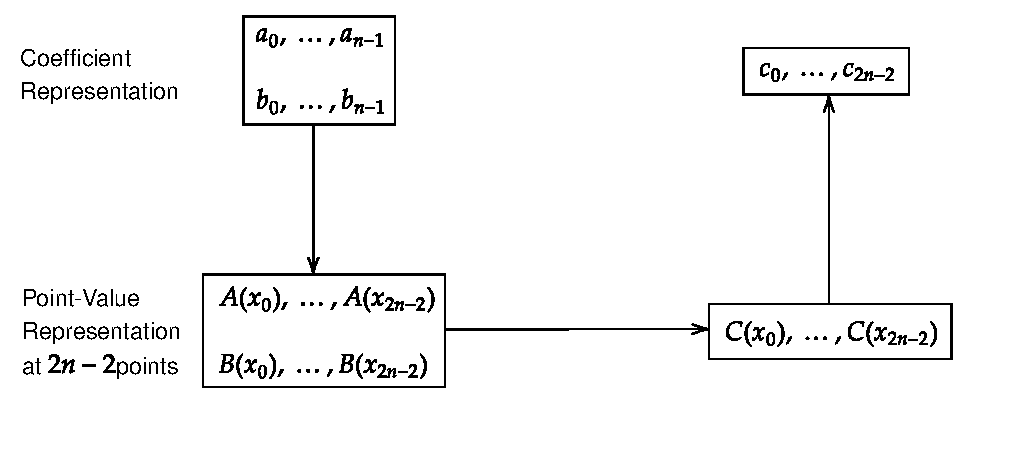
\includegraphics{images/poly-mult}
%\end{figure}
\begin{center}

\begin{tikzpicture}[node distance=3cm, thick]
	
	% Define the rectangles
	\node[draw, rectangle, minimum width=3cm, minimum height=1.5cm] (rect1) at (0, 1.5) {$ \begin{array}{l}
			a_{0} ,\dotsc ,a_{n-1}\\
			\\
			b_{0} ,\dotsc ,b_{n-1}
		\end{array}$};
	\node[draw, rectangle, minimum width=3cm, minimum height=1.5cm] at (0,-3) (rect2) {$ \begin{array}{l}
			A( x_{0}) ,\dotsc ,A( x_{2n-2})\\
			\\
			B( x_{0}) ,\dotsc ,B( x_{2n-2})
		\end{array}$};
	\node[draw, rectangle, minimum width=3cm, minimum height=1cm]  at (8, 1.5) (rect3) {$c_{0} ,\dotsc ,c_{2n-2}$};
	\node[draw, rectangle, minimum width=4cm, minimum height=1.5cm] at (8,-3) (rect4) {$C( x_{0}) ,\dotsc ,C( x_{2n-2})$};
	% Define the text blocks on the left
	\node[align=left] (text1) at (-4, 1.5) {Coefficient\\ Representation};
	\node[align=left] (text2) at (-4, -3) {Point-Value\\ Representation\\ at $\displaystyle 2n-2$ points};
	
	% Draw dotted helper lines (optional for alignment visualization)
	\draw[-Stealth] (rect1.south) -- (rect2.north);
	\draw[-Stealth] (rect2.east) -- (rect4.west);
	\draw[-Stealth] (rect4.north) -- (rect3.south);	
\end{tikzpicture}
\end{center}
\subsection{Finding Evaluations of Multiplied Polynomial}

Suppose we were given $A(x)$ and $B(x)$ evaluated at $2n-1$ distinct points $x_0,\dots, x_{2n-2}$. Then we can get $C(x)$ evaluated at $x_0,\dots, x_{2n-2}$ by $$C(x_i)=A(x_i)B(x_i)\ \forall\ i\in \llbracket 2n-2\rrbracket$$Since there are $O(n)$ many points and for each point it takes constant time to multiply we can find evaluations of $C$ at $x_0,\dots, x_{2n-2}$ in $ O(n)$ time.
\subsection{Evaluation of a Polynomial at Points}\label{fft}
\begin{question}{}{}
	Suppose there is only one point, $x_0$. Can we evaluate a $n-1$ degree polynomial $A(x)=\sum\limits_{i=0}^{n-1}a_ix^i$ at $x_0$ efficiently?
\end{question}
We can rewrite $A(x)$ as $$A(x)=a_0+x(a_1+x(a_2+x(a_3+\cdots (a_{n-1}+x(a_n))\cdots )))$$In this represent it is clear that we have to do $n$ additions and $n$ multiplications to find $A(x_0)$. Hence we can evaluate a $n-1$ degree polynomial at a point in $O(n)$ time


But we have $O(n)$ points. And if each point takes $O(n)$ time to find the evaluation of the polynomial then again it will take total $O(n^2)$ time. We are back to square one. So instead we will evaluate the polynomial in some special points and we will evaluate in all of them in $O(n\log n)$ time. So now the problem we will discuss now is to find some special $n$ points where we can evaluate a $n-1$-degree polynomial in $O(n\log n)$ time.
\parinf

\textbf{Idea:} Evaluate at roots of unity and use Fast Fourier Transform
\parinn

Assume $n$ is a power of 2. NWe have the polynomial $A(x)=\sum\limits_{i=0}^{n-1}a_ix^i$. So now consider the following two polynomials $$A^0(x)=a_0+a_2x+a_4x^2+\cdots+a_{n-2}x^{\frac{n}2-1}\qquad A^1(x)=a_1+a_3x+a_5x^2+\cdots+a_{n-1}x^{\frac{n}2-1}$$Certainly we have $$A(x)=A^0(x^2)+xA^1(x^2)$$Hence we can get $A(1)$ and $A(-1)$ by $$A(1)=A^0(1)+A^1(1)\qquad A(-1)=A^0(1)-A^1(1)$$Hence like this by evaluating two $\frac{n}2-1$ degree polynomials at one point we get evaluation of $A$ at two points. More generally for any $y\geq 0$ we have$$A(\sqrt{y})=A^0(y)+\sqrt{y}A^1(y)\qquad A(-\sqrt{y})=A^0(y)-\sqrt{y}A^1(y)$$So by recursing like this evaluating at $1,-1$ we can get evaluations of $A$ at $n^{th}$ roots of unity.

Let $$\om_n^k=n^{th}\text{ root of unity for }k\in\llbracket n-1\rrbracket = e^{i\frac{k}{n}2\pi}=\cos\lt(\frac{k}{n}2\pi\rt)+i\sin s\lt(\frac{k}{n}2\pi\rt)$$Hence we have \begin{align*}
	A\lt(\om_n^k\rt)&=A^0\lt(\om_n^{2k}\rt)+\om_n^kA^1\lt(\om_n^{2k}\rt)=A^0\lt(\om_{\frac{n}2}^{k}\rt)+\om_n^kA^1\lt(\om_{\frac{n}2}^{k}\rt)\\
	A\lt(-\om_n^k\rt)=A\lt(\om_n^{\frac{n}2+k}\rt)&=A^0\lt(\om_n^{2k}\rt)-\om_n^kA^1\lt(\om_n^{2k}\rt)=A^0\lt(\om_{\frac{n}2}^{k}\rt)-\om_n^kA^1\lt(\om_{\frac{n}2}^{k}\rt)
\end{align*}Hence now we will solve the following problem:
\begin{algoprob}
	\problemtitle{Recursive-DFT}
	\probleminput{$(a_0,\dots, a_{n-1})$ representing $(n-1)-$degree polynomial $A(x)=\sum\limits_{i=0}^{n-1}a_ix^i$}
	\problemquestion{Find the evaluations of the polynomial $A(x)$ in all $n^{th}$ roots of unity}
\end{algoprob}

\vspace*{5mm}\parinf
Since $A^0$ and $A^1$ have degree $\frac{n}2-1$ we can use recursion. Hence the algorithm is 
\begin{algorithm}\SetKwComment{Comment}{// }{}
	\DontPrintSemicolon
	\KwIn{$A=(a_0,\dots, a_{n-1})$ such that $A(x)=a_0+a_1x+\cdots+ a_{n-1}x^{n-1}$}
	\KwOut{$A(x)$ evaluated at $n^{th}$ roots of unity $\om_n^k$ for all $k\in\llbracket n-1\rrbracket$}
	\Begin{
	\If{$n==1$}{\Return{$A[0]$}}
	$A^0\longleftarrow (A[0],A[2],\dots,A[n-2])$\;	
	$A^1\longleftarrow(A[1],A[3],\dots,A[n-1])$\;
	$Y^0\longleftarrow 	\prb{Recursive-DFT}(A^0)$\;
	$Y^1\longleftarrow 	\prb{Recursive-DFT}(A^1)$\;		
	\For{$k=0$ to $\frac{n}{2}-1$}{
		
	$Y[k]\longleftarrow Y^0[k]+\om_n^kY^1[k]$\Comment*{$	A\lt(\om_n^k\rt)=A^0\lt(\om_{\frac{n}2}^{k}\rt)+\om_n^kA^1\lt(\om_{\frac{n}2}^{k}\rt)$}
	$Y\lt[k+\frac{n}{2}\rt]\longleftarrow Y^0[k]-\om_n^{\frac{n}2+k}Y^1[k]$\Comment*{$	A\lt(-\om_n^k\rt)=A^0\lt(\om_{\frac{n}2}^{k}\rt)-\om_n^kA^1\lt(\om_{\frac{n}2}^{k}\rt)$}
}
\Return{Y}
}
		\caption{\prb{Recursive-DFT}$(A)$}
	\end{algorithm}

\textbf{Time Complexity}: $T(n)=2T\lt(\frac{n}2\rt)+O(n)=O(n\log n)$.\parinn

 Therefore we can evaluate a $n-1$ degree polynomial in all the $n^{th}$ roots of unity in $O(n\log n)$ time. Hence with this algorithm we will get evaluations of the polynomial $C(x)=A(x)B(x)$ in all the $2n^{th}$ roots of unity. Now we need to interpolate the polynomial $C(x)$ from its evaluations. We will describe the process in the next subsection.
 \subsection{Interpolation from Evaluations at Roots of Unity}In this section we will show how to interpolate a $n-1$ degree polynomial from evaluations at all $n^{th}$ roots of unity. Previously we had $$\underbrace{\mat{C\lt(\om^0_n\rt)\\ C\lt(\om^1_n\rt)\\ C\lt(\om^2_n\rt)\\ \vdots\\ C\lt(\om^{n-1}_n\rt)}}_{Y}=\underbrace{\mat{1 & \om^0_n & \om ^{0\cdot 2}& \cdots & \om^{0\cdot (n-1)}\\  1 & \om^1_n & \om ^{1\cdot 2}& \cdots & \om^{1\cdot (n-1)}\\ 1 & \om^2_n & \om ^{2\cdot 2}& \cdots & \om^{2\cdot (n-1)}\\ \vdots & \vdots & \vdots & \ddots & \vdots\\ 1 & \om^{n-1}_n & \om ^{(n-1)\cdot 2}& \cdots & \om^{(n-1)\cdot (n-1)}}}_{V=\text{ Vandermonde Matrix}}\underbrace{\mat{c_0\\ c_1\\ c_2\\ \vdots \\ c_{n-1}}}_{C}$$
 
 Now vandermonde matrix is invertible since all the $n^{th}$ roots are distinct. Therefore $C=V^{-1}Y$. But we can not do a matrix inversion to interpolate the polynomial because that will take $O(n^2)$ time. Instead we have this beautiful result:
 \begin{lemma}{}{}
 	$\lt(V^{-1}\rt)_{j,k}=\frac1n\om_n^{-jk}$ for all $0\leq j,k\leq n-1$
 \end{lemma}
\begin{proof}
	Consider the matrix $n\times n$ matrix $T$ such that $(T)_{j,k}=\frac1n\om_n^{-jk}$. Now we will show $VT=I$ This will confirm that $V^{-1}=T$. Now $$\sum_{k=0}^{n-1} (V)_{i,j}\, (T)_{j,k}=\sum_{k=0}^{n-1} \om^{ij}_n\times \frac1n\om_n^{-jk}=\frac1n\sum_{k=0}^{n-1}\lt(\om^{i-k}_n\rt)^j=\begin{cases}
		\dfrac1n\dps{\sum\limits_{k=0}^{n-1}}1=1& \text{when $i=k$}\\[5mm] \dfrac1n \dfrac{1-\om^n_n}{1-\om} =0 & \text{when $i\neq k$}
	\end{cases} $$Hence in $VT$ there are $1'$s on the diagonal and rest of the locations are $0$. Hence $VT=I$. So $V^{-1}=T$.
\end{proof}
Hence we can see the inverse of the vandermonde matrix is also a vandermode matrix with a scaling factor. We will denote $y_i=C\lt(\om_n^{i}\rt)$ for $i\in\llbracket n-1\rrbracket$ since these values are given to us some how and we have to find the corresponding polynomial. Therefore we have $$\underbrace{\mat{c_0\\ c_1\\ c_2\\ \vdots \\ c_{n-1}}}_{C}=\frac1n\underbrace{\mat{1 & 1 & 1& \cdots & 1\\  1 & \om^{-1}_n & \om ^{-1\cdot 2}& \cdots & \om^{-1\cdot (n-1)}\\ 1 & \om^{-2}_n & \om ^{-2\cdot 2}& \cdots & \om^{-2\cdot (n-1)}\\ \vdots & \vdots & \vdots & \ddots & \vdots\\ 1 & \om^{-(n-1)}_n & \om ^{-(n-1)\cdot 2}& \cdots & \om^{-(n-1)\cdot (n-1)}}}_{V^{-1}}\underbrace{\mat{c_0\\ c_1\\ c_2\\ \vdots \\ c_{n-1}}}_{C}\underbrace{\mat{y_0\\ y_1\\ y_2\\ \vdots\\ y_{n-1}}}_{Y}$$
\begin{observation*}
	$nc_j=y_0+y_1\om_n^{-j}+y_2\om_n^{-2j}+\cdots+y_{n-1}\om_n^{-(n-1)j}$ for all $j\in\llbracket n-1\rrbracket$.
\end{observation*}
We can also see this situation as we have the polynomial $Y(x)=y_0+y_1x+y_2x^2+\cdots +y_{n-1}x^{n-1}$ and $c_j$ is just $Y(x)$ evaluated as $\om^{-j}_n=\om_n^{n-j}$ multiplied by $n$. Hence we just reindex the $n^{th}$ roots of unity and evaluate $Y$ $n^{th}$ roots of unity in $O(n\log n)$ time using the algorithm described in \autoref{fft}
\chapter{Longest Increasing Subsequence}
\begin{algoprob}
	\problemtitle{\prb{Longest Increasing Subsequence}}
	\probleminput{Sequence of distinct integers $A=(a_1,\dots, a_n)$}
	\problemquestion{Given an array of distinct integers find the longest increasing subsequence i.e. return maximum size set $S\subseteq[n]$ such that $\forall\ i,j\in S$, $i<j\implies a_i<a_j$}
\end{algoprob}
\dfnc[dynamic-prog]{Dynamic Programming}{Dynamic Programming has 3 components:\begin{enumerate}
		\item {Optimal Substructure}: Reduce problem to smaller independent problems
		\item {Recursion}: Use recursion to solve the problems by solving smaller independent problems
		\item {Table Filling}: Use a table to store the result to solved smaller independent problems.
\end{enumerate}}
\section{$O(n^2)$ Time Algorithm}
Given $A=(a_1,\dots, a_n)$ first we will create a $n$-length array where $i^{th}$ entry stores the length and longest increasing subsequence ending at $a_i$. Certainly we have the following recursion relation$$\prb{LIS}(k)=1+\max\limits_{\substack{j<k,\  a_j<a_k}}\{\prb{LIS}(j)\}$$since if a subsequence $S\subseteq [n]$ is the longest increasing subsequence ending at $a_k$ then certainly $S-\{k\}$ is the longest increasing subsequence which ends at $a_j<a_k$ for some $j<k$. 

Hence in the table we start with 1st position and using the recursion relation we fill the table from left. And after the table is filled we look for which entry of the table has maximum length. So the algorithm will be following:

\begin{algorithm}\SetKwComment{Comment}{// }{}
	\DontPrintSemicolon
	\KwIn{Sequence of distinct integers $A=(a_1,\dots, a_n)$}
	\KwOut{Maximum size set $S\subseteq [n]$ such that $\forall\ i,j\in S$, $i<j\implies a_i<a_j$.}
	\Begin{
	Create an array $T$ of length $n$\;
	\For{$i\in[n]$}{
	$T[i][1]\longleftarrow 1+\max\{T[j][1]\colon j<k,\ a_j<a_k\}$\Comment*{Finds $\prb{LIS}[i]$}
$T[i][2]\longleftarrow T\big[T[i][1]-1\big][2]$
}	
$Index\longleftarrow \max \{T[j][1]\colon j\in[n]\}$\;
\Return{$T[Index]$}
}
\caption{\prb{LIS}$(A)$}
\end{algorithm}
\pagebreak 

For each iteration of the loop it takes $O(n)$ time to find $\prb{LIS}[i]$. Hence the time complexity of this algorithm is $O(n^2)$. 
\section{$O(n\log n)$ Time Algorithm}

\begin{algorithm}\SetKwComment{Comment}{// }{}
	\DontPrintSemicolon
	\KwIn{Sequence of distinct integers $A=(a_1,\dots, a_n)$}	
	\KwOut{Maximum size set $S\subseteq [n]$ such that $\forall\ i,j\in S$, $i<j\implies a_i<a_j$.}
\Begin{
	Create an array $T$ of length $n$ with all entries $0$\;
	Create an array $M$ of length $n$\;
	\For{$i=1,\dots, n$}{$M[i]\longleftarrow \infty$}	
	\For{$i=1,\dots,n$}{
		$k\longleftarrow $Find smallest index $i$ such that $M[k]>a_i$ using \prb{Binary-Search}\;
		$M[k]\longleftarrow i$\;
		$T[i]\longleftarrow M[k-1]$\Comment*{Pointer to the previous element of the sequence}
}
$k_0\longleftarrow $ Largest $k_0$ such that $M[k_0]$ is finite\;
Create an array $S$ of length $k_0$\;
\For{$i=k_0,\dots, 1$}{
	\If{$i=k_0$}{$S[k_0]\longleftarrow M[k_0]$\;
	Continue}
$S[i]\longleftarrow T\big[S[i+1]\big]$\Comment*{$T[S[i+1]]$ is pointer to previous value of sequence}
}
\Return{$(k_0,S)$}
}
\caption{\prb{QuickLIS}$(A)$}
\end{algorithm}
\chapter{Opimal Binary Search Tree}
\chapter{Hoffman Encoding}
%\printbibliography[heading=none]
%\addcontentsline{toc}{chapter}{Bibliography}
%\bibliographystyle{alpha}
%\bibliography{algorithms_refs}
\end{document}
